%%% DOCUMENTCLASS
%%%-------------------------------------------------------------------------------

\documentclass[
    a4paper, % Stock and paper size.
    11pt, % Type size.
    % article,
    % oneside,
    onecolumn, % Only one column of text on a page.
    % openright, % Each chapter will start on a recto page.
    % openleft, % Each chapter will start on a verso page.
    openany, % A chapter may start on either a recto or verso page.
]{memoir}

%%% PACKAGES
%%%------------------------------------------------------------------------------

\usepackage[utf8]{inputenc} % If utf8 encoding
\usepackage[T1]{fontenc}    %
\usepackage[german]{babel} % German if it pleases m'lord
\usepackage[final]{microtype} % Less badboxes
\usepackage{csquotes} % For german quotations
\usepackage{xcolor} % For colors
\usepackage{listings} % For colors
\usepackage{enumitem} % For enumerations

% \usepackage{kpfonts} %Font

\usepackage{bbm}
\usepackage{makecell} % tables cells with line breaks etc.
\usepackage{amsmath,amssymb,mathtools,polynom} % Math
\usepackage{minted} % Source code highlighting
\usepackage[most]{tcolorbox} % For custom example styles
\usepackage{siunitx}

% \usepackage{tikz} % Figures
\usepackage{graphicx} % Include figures

\usepackage{wrapfig} % Wrap text around figures

%%% ENVIROMENT VARIABLES
\ExplSyntaxOn

\usepackage{xparse}

\NewDocumentCommand{\getenv}{om}
{
	\sys_get_shell:nnN { kpsewhich ~ --var-value ~ #2 } { } \l_tmpa_tl
	\tl_trim_spaces:N \l_tmpa_tl
	\IfNoValueTF { #1 }
	{
		\tl_use:N \l_tmpa_tl
	}
	{
		\tl_set_eq:NN #1 \l_tmpa_tl
	}
}

\ExplSyntaxOff


\getenv[\TEXPRINT]{TEXPRINT}
\def\apar{\par}

%%%------------------------------------------------------------------------------


%%% PAGE LAYOUT
%%%------------------------------------------------------------------------------

\raggedbottom
\setlrmarginsandblock{0.1\paperwidth}{*}{1} % Left and right margin
\setulmarginsandblock{0.2\paperwidth}{*}{1}  % Upper and lower margin
\checkandfixthelayout


%%% SECTIONAL DIVISIONS
%%%------------------------------------------------------------------------------

\maxsecnumdepth{subsection} % Subsections (and higher) are numbered
\setsecnumdepth{subsection}

\makeatletter %
\makechapterstyle{standard}{
  \setlength{\beforechapskip}{0\baselineskip}
  \setlength{\midchapskip}{1\baselineskip}
  \setlength{\afterchapskip}{8\baselineskip}
  \renewcommand{\chapterheadstart}{\vspace*{\beforechapskip}}
  \renewcommand{\chapnamefont}{\centering\normalfont\Large}
  \renewcommand{\printchaptername}{\chapnamefont \@chapapp}
  \renewcommand{\chapternamenum}{\space}
  \renewcommand{\chapnumfont}{\normalfont\Large}
  \renewcommand{\printchapternum}{\chapnumfont \thechapter}
  \renewcommand{\afterchapternum}{\par\nobreak\vskip \midchapskip}
  \renewcommand{\printchapternonum}{\vspace*{\midchapskip}\vspace*{5mm}}
  \renewcommand{\chaptitlefont}{\centering\bfseries\LARGE}
  \renewcommand{\printchaptertitle}[1]{\chaptitlefont ##1}
  \renewcommand{\afterchaptertitle}{\par\nobreak\vskip \afterchapskip}
}
\makeatother

\chapterstyle{standard}

\setsecheadstyle{\normalfont\large\bfseries}
\setsubsecheadstyle{\normalfont\normalsize\bfseries}
\setparaheadstyle{\normalfont\normalsize\bfseries}
\setparaindent{0pt}
\setafterparaskip{0pt}
\setlength{\parskip}{0.8em}
\setlength{\parindent}{0pt}


%%% FLOATS AND CAPTIONS
%%%------------------------------------------------------------------------------

\makeatletter                  % You do not need to write [htpb] all the time
\renewcommand\fps@figure{htbp} %
\renewcommand\fps@table{htbp}  %
\makeatother                   %

\captiondelim{\space } % A space between caption name and text
\captionnamefont{\small\bfseries} % Font of the caption name
\captiontitlefont{\small\normalfont} % Font of the caption text

% \changecaptionwidth          % Change the width of the caption
% \captionwidth{1\textwidth} %

%%% ABSTRACT
%%%------------------------------------------------------------------------------

\renewcommand{\abstractnamefont}{\normalfont\small\bfseries} % Font of abstract title
\setlength{\absleftindent}{0.1\textwidth} % Width of abstract
\setlength{\absrightindent}{\absleftindent}

%%% HEADER AND FOOTER
%%%------------------------------------------------------------------------------

\makepagestyle{standard} % Make standard pagestyle

\makeatletter                 % Define standard pagestyle
\makeevenfoot{standard}{}{}{} %
\makeoddfoot{standard}{}{}{}  %
\makeevenhead{standard}{\bfseries\thepage\normalfont\qquad\small\leftmark}{}{}
\makeoddhead{standard}{}{}{\small\rightmark\qquad\bfseries\thepage}
% \makeheadrule{standard}{\textwidth}{\normalrulethickness}
\makeatother                  %

\makeatletter
\makepsmarks{standard}{
    \createmark{chapter}{both}{shownumber}{\@chapapp\ }{ \quad }
    \createmark{section}{right}{shownumber}{}{ \quad }
    \createplainmark{toc}{both}{\contentsname}
    \createplainmark{lof}{both}{\listfigurename}
    \createplainmark{lot}{both}{\listtablename}
    \createplainmark{bib}{both}{\bibname}
    \createplainmark{index}{both}{\indexname}
    \createplainmark{glossary}{both}{\glossaryname}
}
\makeatother                               %

\makepagestyle{chap} % Make new chapter pagestyle

\makeatletter
\makeevenfoot{chap}{}{\small\bfseries\thepage}{} % Define new chapter pagestyle
\makeoddfoot{chap}{}{\small\bfseries\thepage}{}  %
\makeevenhead{chap}{}{}{}   %
\makeoddhead{chap}{}{}{}    %
% \makeheadrule{chap}{\textwidth}{\normalrulethickness}
\makeatother

\nouppercaseheads
\pagestyle{standard}               % Choosing pagestyle and chapter pagestyle
\aliaspagestyle{chapter}{chap} %

%%% NEW COMMANDS
%%%------------------------------------------------------------------------------

% Differential operator
\providecommand\d{}
\renewcommand{\d}[1]{\:\mathrm{d}{#1}}
\newcommand{\pdd}[2]{\frac{\partial #1}{\partial #2}}

% N-th root
% \nroot{3}{27}
\newcommand*{\nroot}[2]{\sqrt[\leftroot{-1}\uproot{2}#1]{#2}}
\newcommand*{\ncroot}[4]{\sqrt[\leftroot{#1}\uproot{#2}#3]{#4}}

% 2 component vector
% \tvect{1}{-1}
% \tvec{1}{-1}
\newcommand{\tvect}[2]{%
   \ensuremath{\Bigl(\negthinspace\begin{smallmatrix}#1\\#2\end{smallmatrix}\Bigr)}}
\newcommand{\tvec}[2]{%
    \ensuremath{\left(\negthinspace\begin{matrix}#1\\#2\end{matrix}\right)}}

% 3 component vector
% \rvect{1}{-1}{0}
% \rvec{1}{-1}{0}
\newcommand{\rvect}[3]{%
   \ensuremath{\Bigl(\negthinspace\begin{smallmatrix}#1\\#2\\#3\end{smallmatrix}\Bigr)}}
\newcommand{\rvec}[3]{%
    \ensuremath{\left(\negthinspace\begin{matrix}#1\\#2\\#3\end{matrix}\right)}}

% German-style quotation marks %
\MakeOuterQuote{"}

% Number sets
\newcommand{\N}{\mathbb{N}}
\newcommand{\Z}{\mathbb{Z}}
\newcommand{\Q}{\mathbb{Q}}
\newcommand{\R}{\mathbb{R}}
\newcommand{\C}{\mathbb{C}}

\newcommand{\setzero}{\varnothing}

% Mention (small caps)
\newcommand{\mention}[1]{\textsc{#1}}

% Units
\newcommand{\ukm}{\text{km}}
\newcommand{\uh}{\text{h}}
\newcommand{\ukmh}{\frac{\ukm}{\uh}}
\newcommand{\degrees}[1]{\SI{#1}{\degree}}

% Floor / ceil
\newcommand{\floor}[1]{\left\lfloor #1 \right\rfloor}
\newcommand{\ceil}[1]{\left\lceil #1 \right\rceil}

\newcommand{\term}[2]{$\stackrel{\hbox{\tiny \textnormal{#2}}}{\hbox{#1}}$}
% \newcommand{\term}[2]{#1}



%%%% NEW ENVIRONMENTS
%%%------------------------------------------------------------------------------

\newenvironment{memo}
{\begin{quote}%
	\large\bfseries}
{\end{quote}}

%%%% NEW THEOREMS
%%%------------------------------------------------------------------------------

\ifx\TEXPRINT\apar
	\newtcbtheorem[list inside={example}]{example}{Beispiel}{
		colback=blue!5!white,
		colbacktitle={blue!25!white},
		coltitle={black},
		fonttitle=\bfseries
	}{ex}

	\newtcbtheorem[list inside={definition}]{definition}{Definition}{
		colback=yellow!20!white,
		colbacktitle={yellow!40!white},
		coltitle={black},
		fontupper=\slshape,
		fonttitle=\bfseries
	}{def}
	
	\newtcbtheorem[list inside={statement}]{statement}{Aussage}{
		colback=red!5!white,
		colbacktitle={red!25!white},
		coltitle={black},
		fontupper=\slshape,
		fonttitle=\bfseries
	}{stmt}
\else
	\newtcbtheorem[list inside={example}]{example}{Beispiel}{
		breakable,
		fonttitle=\bfseries,
		colback=white,
		colbacktitle=white,
		coltitle=black,
		colframe=white,
		boxrule=0mm,boxsep=0mm,
		toprule=0mm,bottomrule=0mm,leftrule=0mm,rightrule=0mm,titlerule=0mm,
		left=0mm,lefttitle=0mm,leftupper=4mm,leftlower=0mm,
		right=0mm,righttitle=0mm,rightupper=0mm,rightlower=0mm,
		top=4mm,toptitle=0mm,
		bottom=0mm,bottomtitle=0mm,
		middle=0mm
	}{ex}
	
	\newtcbtheorem[list inside={definition}]{definition}{Definition}{
		breakable,
		colback=white,
		colbacktitle=white,
		coltitle=black,
		colframe=white,
		fontupper=\slshape,
		fonttitle=\bfseries,
		boxrule=0mm,boxsep=0mm,
		toprule=0mm,bottomrule=0mm,leftrule=0mm,rightrule=0mm,titlerule=0mm,
		left=0mm,lefttitle=0mm,leftupper=4mm,leftlower=0mm,
		right=0mm,righttitle=0mm,rightupper=0mm,rightlower=0mm,
		top=4mm,toptitle=0mm,
		bottom=0mm,bottomtitle=0mm,
		middle=0mm
	}{def}
	
	\newtcbtheorem[list inside={statement}]{statement}{Aussage}{
		breakable,
		colback=white,
		colbacktitle=white,
		coltitle=black,
		colframe=white,
		fontupper=\slshape,
		fonttitle=\bfseries,
		boxrule=0mm,boxsep=0mm,
		toprule=0mm,bottomrule=0mm,leftrule=0mm,rightrule=0mm,titlerule=0mm,
		left=0mm,lefttitle=0mm,leftupper=4mm,leftlower=0mm,
		right=0mm,righttitle=0mm,rightupper=0mm,rightlower=0mm,
		top=4mm,toptitle=0mm,
		bottom=0mm,bottomtitle=0mm,
		middle=0mm
	}{stmt}

\fi

%%% TABLE OF CONTENTS
%%%------------------------------------------------------------------------------

\maxtocdepth{section} % Only parts, chapters and sections in the table of contents
\settocdepth{section}

\AtEndDocument{\addtocontents{toc}{\par}} % Add a \par to the end of the TOC

%%% INTERNAL HYPERLINKS
%%%-------------------------------------------------------------------------------

\usepackage{hyperref}   % Internal hyperlinks
\ifx\TEXPRINT\apar
	\hypersetup{
		colorlinks,
		linkcolor={red!50!black},
		citecolor={blue!50!black},
		urlcolor={blue!80!black},
		pdfauthor={Andre Wachsmuth}
	}
\else
	\hypersetup{
		hidelinks,
		pdfauthor={Andre Wachsmuth}
	}
\fi
\usepackage{memhfixc}   %

%%% Colors
%%%-------------------------------------------------------------------------------
\definecolor{LightGray}{rgb}{0.95,0.95,0.95}


%%% SOURCE CODE
%%%-------------------------------------------------------------------------------

% Default for all source code listings
\setminted{
	framesep=2mm,
	baselinestretch=1.0,
	bgcolor=LightGray,
	fontsize=\footnotesize,
	linenos
}

% specific languages
\newminted{c}{}
\newminted{js}{}
\newminted{text}{}

% polynomial long division
\polyset{%
    style=C,
    delims={\big(}{\big)},
    div=:
}

%%%% Named equations
%%%------------------------------------------------------------------------------
% Define Nequation environment for named equations.
% This is based on
%     http://tex.stackexchange.com/questions/128050/add-equation-name-underneath-equation-number
\usepackage{stackengine}
\def\stackalignment{r}
\def\stacktype{L}
\def\useanchorwidth{T}
% From page 3 of
%     http://tug.ctan.org/macros/latex/contrib/stackengine/stackengine.pdf
\def\Lstackgap{0.666666\baselineskip}
\newlength\eqshift
\setlength\eqshift{\widthof{)}}
\let\savetheequation\theequation
\newenvironment{Nequation}[1]%
{%
	\def\thecurrentname{#1}%
	\let\theequation\savetheequation
	\begin{equation}%
	\renewcommand\theequation
	{%
		\stackunder
		{\savetheequation}%
		{{\thecurrentname}\hspace{-\eqshift}}%
	}%
}%
{%
	\end{equation}%
	\addcontentsline{loe}{equation}{\protect\numberline{\theequation}\thecurrentname}%
	\let\theequation\savetheequation
	\ignorespacesafterend
}


\author{Andre Wachsmuth}
\title{Analysis / Infinitesimalrechnung}

\usepackage{lipsum} % Just to put in some text

\begin{document}

\frontmatter

\maketitle

\begin{abstract}

Begleitende Notizen für die Modulvorlesung Analysis im Studiengang Informationstechnologie an der Berufsakademie Sachsen. Ziel ist die Einführung in die höhere Mathematik, speziell in die Theorie der Infinitesimalrechnung und Differenzgleichungen in Hinblick auf die Modellierung von physikalischen und anderen Sachverhalten. Es wird vorausgesetzt, dass grundlegende Kenntnisse aus der Mathematikausbildung der Seminarstufe I und II vorhanden sind.

\end{abstract}

\clearpage

\tableofcontents*
\clearpage

\chapter{Einführung}

\section{Organisatorisches}

\begin{itemize}
	\item Klausur: Schriftlich, 2 Stunden, davon $\frac{1}{3}$ Analysis, $\frac{2}{3}$ Algebra
	\item Hilfsmaterialen: Kein Taschenrechner, jeweils 1 handbeschriebenes A4-Blatt
	\item Online-Materialen: \href{https://drive.google.com/drive/folders/1CJ0226zg1_bnbt7IopCLwDuK2hkOgHya?usp=sharing}{drive.google.com}
	\item \LaTeX-Quellcode und weiteres: \href{https://github.com/blutorange/ba-dresden-calculus-awa}{github:blutorange/ba-dresden-calculus-awa}
	\item Kontakt: \href{mailto:wachsmuth.andre@gmx.de?subject=BA/Analysis 2020: }{wachsmuth.andre@gmx.de}
	\item Buchempfehlung: Meyers kleine Enzyklopädie der Mathematik, hrsg. von Siegried Gottwald, Meyers Lexikonverlag, \href{https://www.amazon.de/-/en/Siegfried-Gottwald/dp/3411077719}{ISBN-3 3-411-07771-9}
	\item Buchempfehlung: Repetitorium der höheren Mathematik, Merziger / Wirth, Binomi-Verlag, \href{https://www.amazon.de/-/en/Gerhard-Merziger/dp/3923923333}{ISBN-3 3-923-923-33-3}
\end{itemize}

\section{Anwendungen der Mathematik}

Mathematik stärkt die Fähigkeit zur Abstraktion und hilft bei der Lösung komplexer, auch nicht-mathematischer, Probleme. Grundlegend
ist die Fähigkeit, ein Problem analysieren zu können, es in Unterprobleme zu teilen und eine Lösungsstrategie zu erarbeiten zu können.

Auch in der Informatik und Programmierung sind mathematische Konzepte in einem breiten Umfang relevant.

\begin{itemize}
	\item In der objektorientierten Programmierung gibt es den Begriff der "Datenklassen". Um zu definieren, wie man diese vergleicht (\#equals) und ordnet (\#compareTo), werden Konzepte aus der Theorie der Relationen benötigt.
	\item Die Graphentheorie spielt eine wichtige Rollen bei Datenstrukturen und Algorithmen. Binäre Bäume stellen eine wichtige Datenstruktur für die effiziente Berechnung dar, gewichtete Graphen sind von wichtiger Bedeutung für das Problem des Handelsreisenden (Traveling Salesman), welches Anwendung findet in der Routenplanung, der Netzwerkarchitektur oder der Schaltkreisplanung.
	\item Grenzwertbetrachtungen und sogenannte Landau-Symbole werden genutzt, um die Laufzeit und den Speicherverbrauch von Algorithmen zu analysieren und zu beschreiben.
	\item Die Kategorientheorie ist eine Grundlage für algebraische Datenstrukturen. Zusammen mit dem $\lambda$-Kalkül stellen Sie die Basis funktionaler Programmierung dar.
	\item Die kontinuierliche Mathematik und die Infinitesimalrechnung stellen den Grundbaustein dar für physikalische Simulationen (Windtunnel, Crash-Test, Physics-Engine) und computergestützte Ingenieurswissenschaften (Gebäudestatik, Hydrodynamik, Schaltkreissimulation).
\end{itemize}

\section{Zahlenbereiche}

Grundlage für die gesamte Analysis die Objekte, auf denen sie operiert: Zahlen und Zahlenmengen. Zahlen modellieren quantitative Zusammenhänge der realen Welt. Gleichartige Zahlen abstrahiert man als eine Menge zu Zahlenbereichen.


\begin{definition}{Menge}{Set}
	Eine \textbf{Menge} ist eine Sammlung verschiedenartiger Elemente. Irrelevant hierbei ist die Reihenfolge der Elemente.
\end{definition}

Bei obiger Definition handelt es sich um den sogenannten naiven Mengenbegriff. Es hat sich gezeigt, dass diese naive Vorstellung zu Widersprüchen führen kann,
weshalb präzisere Formulierungen der Mengentheorie gefunden wurden (etwa Zermelo–Fraenkel-Mengenlehre). Für diese Vorlesung ist der naive Mengenbegriff allerdings
ausreichend.

Bei der Definition der Zahlenbereich beginnt man mit den natürlichen Zahlen und erweitert diese dann schrittweise.

\begin{definition}{Natürliche Zahlen}{NatNum}
	Die \textbf{natürlichen Zahlen} sind die Menge $\N$, die man erhält, wenn man mit dem Element $0$ beginnt und weitere Elemente rekursiv durch Bildung des Nachfolgers bestimmt.
\end{definition}

Präzisiert wird diese Definition durch die sogenannten \mention{Peano}-Axiome. Dabei kann man $0$ etwa mit dem Element $\setzero$ (leere Menge) identifzieren und die Nachfolgerbildung mit der Zuweisung
$\setzero \mapsto \lbrace \setzero \rbrace$ (Menge mit der leeren Menge). Der Vollständigkeit halber seien diese Axiome hier kurz angegeben.

\begin{definition}{\mention{Peano}-Axiome}{PeanoAx}
	\begin{enumerate}
		\item 0 ist eine Zahl.
		\item Jede Zahl $n$ hat genau einen Nachfolger $n'$.
		\item $0$ ist nicht Nachfolger einer Zahl.
		\item Jede Zahl ist Nachfolger höchstens einer Zahl.
		\item Von allen Mengen, die die Zahl $0$ und mit der Zahl $n$ auch deren Nachfolger $n'$ enthalten, ist die Menge $\N$ der natürlichen Zahlen diejenige mit den wenigsten Elementen.
	\end{enumerate}
\end{definition}

Natürliche Zahlen gibt es in zwei Ausprägungen. Die sogenannten \mention{Kardinalzahlen} beschreiben eine Anzahl, etwa die Anzahl von Büchern in einem Korb oder die Elemente in einem Array (Array-Länge).
Hinzu kommen die $\mention{Ordinalzahlen}$, welche eine Ordnung oder Rangfolge beschreiben. Im Gegensatz zu den Kardinalzahlen kann der Anfang bei Ordinalzahlen beliebig gewählt werden. Man kann den Index eines
Arrays sowohl bei $0$ als auch bei $1$ beginnen lassen, in beiden Fällen wird damit das \emph{erste} Element bezeichnet.

Nun reichen die natürlichen Zahlen nicht aus, um alle Gegebenheiten zu modellieren. Etwa ist es damit umständlich, Einnahmen und Kosten zu beschreiben. Hier müsste man immer angeben, ob es sich bei einer Quantität umd Einnahmen oder Kosten handelt und Regeln festlegen, wie Einnahmen und Kosten miteinander zu verrechnen sind. Um solche Gegensätze besser beschreiben zu können, führt man die ganzen Zahlen ein.
Kosten sind nun einfach beschreibbar als negative Einnahmen. Mathematisch motiviert werden die ganzen Zahlen, um ein inverses Element bezüglich der Addition angeben zu können. Dies wird unter dem Themengebiert siehe algebraische Strukturen im Modul Algebra näher beleuchtet.

\begin{definition}{Ganze Zahlen}{WholeNum}
	Die \textbf{ganzen Zahlen} sind die Menge $\Z$, die man aus $\N$ gewinnt, wenn man zu jeder natürlichen Zahl $n$ noch ihr Inverses $n'$ hinzunimmt. Dabei gilt $n+n' = n+(-n) = 0$.
\end{definition}

Doch auch die ganzen Zahlen sind unzureichend, um Verhältnisse und Verteilungen. Um etwa die Verteilung eines Geburtstagskuchen zu beschreiben, muss man immer die Grundgesamtheit (12 Stücke) als auch den Anteil
davon (3 Stück) angeben. Dies ist umständlich, stellt aber die Idee für die Definition der gebrochenen Zahlen dar.

\begin{definition}{Gebrochene Zahlen}{RatNum}
	Die \textbf{gebrochenen Zahlen} sind die Menge $\Q$, welche aus Paaren $(p,q) \in \Z^2$ ganzer Zahlen besteht. $p$ bezeichnet man dabei als Zähler, $q$ als Nenner. Zwei ganze Zahlen heißen äquivalent,  wenn
	diese den gleichen Bruch darstellen, also wenn gilt: $(p,q) \equiv (p',q') \iff pq'=p'q$
\end{definition}

Solche Brüche werden in der Informatik verwendet, um Fehler bei der Addition und Multiplikation zu vermeiden. Dies ist für einige Anwendungsbereiche wie Finanzen von wichtiger Bedeutung, um Geldbeträge
Cent-genau berechnen zu können. Ein Spezialfall davon ist die sogenannte Festkommazahlrechnung (fixed-point arithmetics), wobei der Nenner immer fest vorgeben ist.

Nun gibt es auch Rechenaufgaben, die selbst durch gebrochene Zahlen nicht gelöst werden können. Beispielsweise hat $x^2=2$ keine Lösung im Bereich der gebrochenen Zahlen. Allerdings ist es möglich,
Näherungswerte als Brüche anzugeben: $\frac{3}{2}, \frac{17}{12},\frac{577}{408}$. Man sieht hier, dass die Näherungswerte besser werden, also näher an der gesuchten Lösung liegen. Tatsächlich kann man
eine Formel angeben, um immer bessere Näherungswerte für $x^2=2$ zu finden. Alle diese Näherungswerte sind gebrochene Zahlen, dennoch gibt es keine gebrochene Zahl mit der Eigenschaft $x^2=2$.

\begin{definition}{Fundamentalfolge}{CauchySeq}
	Eine \textbf{Fundamentalfolge} (Cauchy-Folge) ist eine Zahlenfolge $a_i$, bei der der Abstand zweier Folgenglieder beliebig klein wird:

    \begin{equation}
        \forall \epsilon > 0: \exists N \in \N: \forall m,q>N: |a_m-a_q|<\epsilon
    \end{equation}
\end{definition}

Wie eben anhand des Beispiels $x^2=2$ illustriert, gibt es im Bereich der rationalen Zahlen Fundamentalfolgen, die sich zwar scheinbar einem Wert zu nähern scheinen (die also eine Cauchy-Folge darstellen),
wobei dieser Wert selber allerdings keine gebrochene Zahl ist. Zur Lösung dieses Problems werden die reellen Zahlen definiert.

\begin{definition}{Reelle Zahlen}{RealNum}
	Die \textbf{reellen Zahlen} sind die Menge $\R$, welche aus allen Fundamentalfolgen $a_i$ ganzer Zahlen besteht. Zwei Fundamentalfolgen $a_i, b_i$ sind dabei äquivalent, wenn $|a_i-b_i|$ eine Nullfolge bildet.
\end{definition}

Tatsächlich lässt sich zeigen, dass auf der Menge der reellen Zahlen $\R$ jede Cauchy-Folge konvergiert, also einen Grenzwert besitzt. Die reellen Zahlen sind im Gegensatz zu den gebrochenen Zahlen \emph{vollständig}.

Als Erweiterung der reellen Zahlen gibt es noch die komplexen Zahlen $\C$, wobei ein neues Element $j$ mit der Eigenschaft $j^2=-1$ eingeführt wird, welches die sogenannte imaginäre Einheit heißt. Komplexe
Zahlen eignen sich beispielsweise, um Schwingungen zu beschreiben oder Strom- und Spannungsberechnungen an Schaltkreisen anzustellen. Solche komplexen Zahlen werden in der Algebra genauer betrachtet. Diese Vorlesung beschränkt sich auf die reellwertige Analysis.

\section{Operationen und Rechenregeln}

Auf den Zahlenbereichen werden Rechenoperationen definiert, welche gewisse Regeln genügen. Die systematische Beschreibung solcher Rechenoperationen erfolgt durch das Gebiet algebraische Strukturen im Modul Algebra. Für die Analysis wird vorausgesetzt, dass elementare Rechenregeln aus Sekundarstufe I und II sowie der Umgang und die Umformung mathematischer Terme beherrscht werden. Im folgenden findet sich eine unvollständige Auflistung einiger wesentlicher Regeln:

\begin{statement}{Kommutativgesetz}{CommLaw}
	Für $a,b\in\R$ gilt: $a + b = b + a$
\end{statement}

\begin{statement}{Assoziativgesetz}{AssLaw}
	Für $a,b\in\R$ gilt: $a + ( b + c) = (a + b) + c$
\end{statement}

\begin{statement}{Distributivgesetz}{DisLaw}
	Für $a,b,c\in\R$ gilt: $a \cdot ( b + c ) = a \cdot b + a \cdot c$
\end{statement}

\begin{statement}{Potenzgesetze}{PowerIds}
	Für $x, y, p,q\in\R$, für welche die Potenzen erklärt sind, gelten die folgenden Rechenregeln:
	\begin{itemize}
		\item $x^{p+q} = x^p \cdot x^q$
		\item $x^p \cdot y^p = (x \cdot y)^p$
		\item $x^{(y^z)} = x^{y \cdot z}$
	\end{itemize}
\end{statement}

\begin{statement}{Logarithmengesetze}{LogIds}
	Für $x, y\in\R$, für welche die Logarithmen erklärt sind, gelten die folgenden Rechenregeln:
	\begin{itemize}
		\item $\ln(x \cdot y) = \ln(x) + \ln(y)$
		\item $\ln(x^y) = y \ln(x)$
		\item $\log_y(x) = \ln(x) / \ln(y)$
	\end{itemize}
\end{statement}

Für die Operationen $+$ (Addition) und $*$ (Multiplikation) gibt es zudem eine Kurzschreibweise, wenn eine (möglicherweise variable) Anzahl von Summanden addiert oder Faktoren multipliziert werden sollen. Man gibt dabei einen Laufindex an, der innerhalb gewisser Grenzen verläuft, und einen Term, in den jeder erlaubte Wert des Laufindex eingesetzt wird. Die Werte des Terms für jeden Laufindex werden dann addiert beziehungsweise multipliziert. Geschrieben wird dies wie folgt:

$$
\sum\limits_{i=1}^{10} i^2  \\
$$

$$
\prod\limits_{i=1}^{5} i
$$

Oben steht eine Summe ($\Sigma$ für Sigma, Summe), gesprochen: "Die Summe von i gleich 1 bis 10 über i-Quadrat." Es sollen also die ersten 10 Quadratzahlen addiert werden. Unten steht ein Produkt ($\Pi$ für Pi, Produkt), gesprochen: "Das Produkt von i gleich 1 bis 5 über i." Hier sollen also die Zahlen von $1$ bis $5$ multipliziert werden ($=5!$). Man beachte auch die Analogie zu einer \emph{For-Schleife} in der Programmierung:

\begin{jscode}
sum = 0;
for (i = 1; i <= 10; ++i)
	sum += i * i;
\end{jscode}

\section{Schlussfolgern}

Ein in der Schulmathematik häufig vernachlässigter wichtiger Bestandteil der Mathematik ist das Schlussfolgern, also dem Ziehen von Schlüssen basierend auf gewissen Grundannahmen oder Axiomen. Hierfür
gibt es einige wichtige Techniken wie \emph{Induktion} oder \emph{reductio ad absurdum}. Auch wenn das Beweisführen in dieser Vorlesung nicht im Vordergrund steht, wird erwartet, dass zu einer Antwort
immer eine knappe, aber fundierte Begründung (Rechenweg oder Prosa) gegeben wird. In folgenden wird anhand einiger Beispiele kurz illustriert, wie mathematische Beweise geführt werden können.

\subsection{Beweis durch Widerspruch}

Frage: Ist $\sqrt{2}\in\Q$?

Wir nehmen an, $\sqrt{2}$ wäre eine gebrochene Zahl, also darstellbar als vollständig gekürzter Bruch $\frac{p}{q}, p,q\in\Z, p,q>0$. Dann sind $p$ und $q$ teilerfremd. Es folgt nun:

\begin{align}
  \sqrt{2} & = p / q \\
         2 & = p^2 / q^2 \\
     2 q^2 & = p^2 \label{eq:sqrt2-p2even}
\end{align}

Aus Gleichung \ref{eq:sqrt2-p2even} folgt, $p^2$ ist eine gerade Zahl, da es sich als das doppelte einer anderen ganzen Zahl $q^2$ darstellen lässt. Weiterhin ist damit auch $p$ eine gerade Zahl, da das Produkt zweiter ungerade Zahlen
immer ebenfalls eine ungerade Zahl ergibt. Wir können $p$ nun schreiben als $p = 2 n, n\in \Z$. Es ergibt sich:

\begin{align}
	2q^2 & = p^2 = p * p = (2n) \cdot (2n) \\
	q^2 & = 2 n^2 \label{eq:sqrt2-q2even}
\end{align}

Da $n$ eine ganze Zahl ist, so ist auch $n^2$ eine ganze Zahl. Wegen \ref{eq:sqrt2-q2even} lässt sich $q^2$ sich schreiben als das doppelte einer ganzen Zahl und ist daher eine gerade Zahl, mithin ist also auch $q$ eine gerade Zahl.

Nun haben wir damit aber gezeigt, dass sowohl $p$ als auch $q$ gerade Zahlen sind. Sie besitzen also beide den Teiler $2$. Dies widerspricht der Annahme, dass es einen vollständig gekürzten Bruch $p / q = \sqrt{2}$ gibt. Die Annahme, dass es einen solchen Bruch gibt, wurde damit zu einem Widerspruch (ad absurdum) geführt (reductio). Somit gibt es keine gebrochene Zahl $x$ mit der Eigenschaft $x^2=2$.

\subsection{Nichtkonstruktiver Beweis}

Frage: Gibt es zwei irrationale Zahlen $x,y\notin \Q$ so, dass deren Potenz $x^y\in \Q$ eine rationale Zahl ergibt?

Wir wählen $x=y=\sqrt{2}$. Nach dem Satz vom ausgeschlossenen Dritten ist eine Aussage entweder wahr oder falsch, das heißt entweder gilt $\sqrt{2}^{\sqrt{2}} \in \Q$ oder $\sqrt{2}^{\sqrt{2}}\notin\Q$. Wir betrachten beide Fälle:

\begin{itemize}
	\item $\sqrt{2}^{\sqrt{2}}\in\Q$: $\sqrt{2}$ ist wie eben gezeigt irrational, damit ist ein Beispiel für zwei solche Zahlen gefunden.

	\item $\sqrt{2}^{\sqrt{2}}\notin\Q$: Wir setzen $x' = \sqrt{2}^{\sqrt{2}}$ und $y'=\sqrt{2}$. Die Zahl $x'$ ist nach Annahme irrational und die Potenz $(\sqrt{2}^{\sqrt{2})^{\sqrt{2}}} = \sqrt{2}^{\sqrt{2}\sqrt{2}} = \sqrt{2}^2 = 2$ ist eine rationale Zahl.
\end{itemize}

Wir haben damit gezeigt, dass es wenigstens eine Paar zwei solcher Zahlen gibt, nämlich entweder $(x,y) = (\sqrt{2}, \sqrt{2})$ oder $(x,y) = (\sqrt{2}^{\sqrt{2}}, \sqrt{2})$. Dieser Beweis heißt deshalb nichtkonstruktiv, da er keine Möglichkeit bietet, zu bestimmen, welche Zahlen es tatsächlich sind.

\section{Struktur von Termen}

Um mathematische Ideen zu kommunizieren, ist eine Notation notwendig, die gewissen Regeln folgt. Um etwa die Idee zu beschreiben, dass die Summe zweier Zahlen in einer Menge enthalten sei, wird in der üblichen mathematischen Notation die Schreibweise $a+b\in\N$ verwendet. Wir an diesem Beispiel zu sehen, besteht die mathematische Notation also zum Einen aus Symbolen für mathematische Objekte und Operationen und zum Zweiten aus Regeln, wie diese Symbole angeordnet werden dürfen. Genau dies ist aber die Definition einer sogenannten \emph{formalen Sprache} mit Wörtern und einer Grammatik für die Bildung von Sätzen.

Man beachte die Analogie zu Programmiersprachen, auch diese stellen eine solche formale Sprache dar. Genauso wie ein Programm dargestellt werden kann als \emph{Syntaxbaum} ist dies auch mit einem mathematischen Ausdruck möglich. Ein Syntaxbaum beginnt immer an der Spitze mit der hauptsächlichen Operation, und verzweigt dann in die einzelnen Unteroperation. Wir betrachten als Beispiel zuerst das folgende Computerprogramm zur Berechnung der $n$.-ten Fibonacci-Zahl in Listing \ref{lst:JsFibonacci}.

\begin{listing}[H]
\caption{JavaScript-Programm zur Berechnung der n.-ten Fibonacci-Zahl}
\label{lst:JsFibonacci}
\begin{jscode}
function fibonacci(n) {
	let n_0 = 0;
	let n_1 = 1;
	while (n-- > 0) {
		const sum = n_0 + n_1;
		n_0 = n_1;
		n_1 = sum;
	}
	return n_0;
}
\end{jscode}
\end{listing}


In oberster Ebene ist die Struktur dieses Programms eine \emph{Function Declaration}, bestehend aus einem Funktionsnamen, einem Argument und einem Funktionskörper. Der Funktionskörper selbst ist zuallererst ein \emph{Block Statement}, bestehend aus einer \emph{Statement List}. Das Statement auf Zeile 5, \lstinline{const sum = n_0 + n_1}, wiederum ist ein \emph{Variable Declaration}-Statement, bestehend aus einem \emph{Identifier} für den Variablennamen und einem \emph{Initializer} für den Wert der Variablen. Der \emph{Initializer} ist eine \emph{Sum Expression} (Summen-Ausdruck), der wiederum aus 2 Summanden besteht. Jeder Summand ist in diesem Fall ein \emph{Identifier} für den jeweiligen Variablennamen. Verbal formuliert mag diese Struktur nur schwer vorstellbar sein. Graphisch ist der Syntaxbaum auszugsweise in Abbildung \ref{fig:JsFibinacciBaumPart} dargestellt. Der vollständige Syntaxbaum findet sich in Abbildung \ref{fig:JsFibinacciBaum}.


\begin{figure}[h]
	\caption{Syntaxbaum zum JavaScript-Programm für Fibonacci-Zahlen (Auszug)}
	\label{fig:JsFibinacciBaumPart}
	\centering
	\includegraphics[width=0.5\textwidth]{./img/js-tree-fibonacci-part.png}
\end{figure}


\begin{figure}[p]
	\caption{Syntaxbaum zum JavaScript-Programm für Fibonacci-Zahlen}
	\label{fig:JsFibinacciBaum}
	\centering
	\includegraphics[width=0.95\textwidth]{./img/js-tree-fibonacci.png}
\end{figure}

Für die mathematische Notation besonders relevant sind die Ausdrücke (\emph{Expression}), also Rechenoperationen. Einen mathematischer Term lässt wie erwähnt als Syntaxbaum darstellen. Solch ein Syntaxbaum lässt sich schriftlich auf verschiedene Weisen schreiben. Die mathematische Notation lehnt sich an der sogenannten Infix-Notation an, wobei die Operatoren zwischen die Operanden geschrieben werden. Eine weitere Notation stellt die Polnische Notation dar, die etwa in manchen Taschenrechner verwendet wird und auch die Grundlage für \mention{Ldap}-Filter darstellt (Lightweight Directory Access Protocol). Wir wollen dies kurz am Beispiel $(a+b)\cdot(c+d)$ illustrieren. Der Syntaxbaum dazu ist zu finden in Abbildung \ref{fig:JsAbcdBaum}.

\begin{figure}[H]
	\caption{Syntaxbaum für $(a+b)(c+d)$}
	\label{fig:JsAbcdBaum}
	\centering
	\includegraphics[width=0.5\textwidth]{./img/js-tree-abcd.png}
\end{figure}

Aus dem Syntaxbaum lesen wir ab, dass der Term aus der Hauptoperation \emph{Multiplikation} besteht. Die beiden Faktoren bestehen jeweils aus einer Unteroperation, hier einen Summenbildung. Die Infix-Notation $(a+b)\cdot(c+d)$ beginnt daher mit einem Multiplikationszeichen, zu dessen beiden Seiten Summenzeichen stehen. Um die Rangfolge zu wahren, welche durch den Syntaxbaum vorgegeben ist, erfordert die Infix-Notation die Verwendung von Klammerzeichen. Eine Alternative zur Infix-Notation ist die polnische Notation, welche keine Klammerzeichen benutzt und so etwa einfacher von Computerprogramme verstanden werden kann. Dies erreicht sie dadurch, indem sie zuerst für jeden Operator definiert, welche Arität (Anzahl von Operanden) er hat. Anschließend wird der Operator nicht zwischen die Operanden, sondern vor die Operanden geschrieben. Zusätzlich gibt es noch die sogenannte umgekehrte polnische Notation, wobei der Operator nicht vor, sondern nach den Operanden notiert wird. Für unser Beispiel $(a+b)(c+d)$ ist die polnische Notation dargestellt in Listing \ref{lst:PolAbcd}.

\begin{listing}[H]
	\caption{Polnische Notation (oben) und umgekehrte polnische Notation (unten)}
	\label{lst:PolAbcd}
\begin{textcode}
* + a b + c d
a b + c d + *
\end{textcode}
\end{listing}

Schließlich sei noch angemerkt, dass Rechenregeln sich darstellen lassen als Transformationen auf einem Syntaxbaum. Dies stellt die Grundlage dar für Computer-Algebra-System, welche auf symbolischen Ausdrücken arbeiten und diese umformen können. Dies ist in Abbildung \ref{fig:TreeTransformKommutativ} am Beispiel des Kommutativgesetzes dargestellt. Dieses besagt, dass bei einer \emph{Sum Expression} die beiden Unterbäume der beiden Summanden vertauscht werden können. Man beachte, dass die Summanden im Allgemeinen nicht Zahlen oder Variablen, sondern wiederum komplexe Baumstrukturen sind.

\begin{figure}[H]
	\caption{Syntaxbaumtransformation für das Kommutativgesetz}
	\label{fig:TreeTransformKommutativ}
	\centering
	\includegraphics[width=0.8\textwidth]{./img/tree-transform.png}
\end{figure}

\mainmatter

% Sequences, sums, limit (definition), convergence criteria
\chapter{Zahlenfolgen, Zahlenreihen, Konvergenz}

Der moderne Grenzwertbegriff stellt die Grundlage der Infinitesimalrechnung dar. In diesem Kapitel betrachten wir zuerst Zahlenfolgen und Reihen, definieren dann Konvergenz sowie Grenzwert und lernen abschließend
einige wichtige Regeln zur Konvergenz und Grenzwertbestimmung kennen.

Um die Wichtigkeit zu illustrieren, warum eine exakte Definition der Konvergenz notwendig, sei Zenons Paradoxon von Achilles und der Schildkröte angeführt. \emph{Zeno of Elea} (etwa 500 BC) hat dieses Paradoxon angeführt, um zu zeigen, dass der naive Begriff von Wandel und Bewegung nur eine Illusion wäre. Zur besseren Veranschaulichung wählen für die folgende Erklärung (willkürlich gewählte) Größenabgaben. In dem Paradox nun veranstalten Achilles und eine Schildkröte ein Wettrennen, wie in Abbildung \ref{fig:ZenoAchilles} dargestellt. Achilles ist in der Lage, mit einer Geschwindigkeit von $25\ukmh$ zu rennen, während die Schildkröte nur $5\ukmh$ schafft. Der Fairness halber erhält die Schildkröte daher einen Vorsprung von $100\ukm$. Die Frage ist nun, wann Achilles die Schildkröte überholt. Der geläufige physikalische Ansatz wäre, ein Koordinatensystem zu definieren, die Bewegungsgleichungen beider Partizipanten aufzustellen und den Schnittpunkt zu berechnen. Zenon argumentiert allerdings wie folgt:

\begin{enumerate}
	\item Damit Achilles die Schildkröte überholen kann, muss er zunächst den Vorsprung von $100\ukm$ aufholen. Dazu benötigt er $4$ Stunden.
	\item In diesen $4$ Stunden allerdings ist die Schildkröte bereits $20\ukm$ weiter gekrochen.
	\item Also muss Achillles im nächsten Schritt diese $20\ukm$ Vorsprung aufholen, wozu er $0.8$ Stunden benötigt. Aber nun hat die Schildkröte bereits einen neuen Vorsprung erhalten.
	\item Egal, wie oft Achilles also den Vorsprung aufholt, um die Schildkröte zu überholen, müsste er unendliche viele Vorsprünge aufholen. Also holt Achilles die Schildkröte nie ein, um kann sie somit auch nicht überholen.
\end{enumerate}

Wie lässt sich dieses Paradoxon auflösen? Der Fehler, den Zenon hier begeht, besteht darin, dass Achilles zum Aufholen "unendlicher" vieler Vorsprünge auch "unendlich" viel Zeit benötigt. Dies ist aber bei einer genauen Betrachtung mithilfe eines exakten Grenzwertbegriffs nicht der Fall, wie wir auch in einer Übungsaufgabe nachweisen werden.

\begin{figure}[H]
	\caption{Zenos Paradoxon von dem Wettrennen zwischen Achilles und der Schildkröte}
	\label{fig:ZenoAchilles}
	\centering
	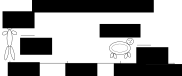
\includegraphics[width=0.95\textwidth]{./svg/zeno-achilles.png}
\end{figure}



\section{Zahlenfolgen und Reihen}

Bevor wir den Begriff der Konvergenz näher definieren können, benötigen wir zuerst ein Verständnis von Zahlenfolgen.

\begin{definition}[Unendliche Zahlenfolge]
	Eine unendliche Zahlenfolge ist gegeben, wenn jeder natürlichen Zahl $n \ge 0$  genau eine (meist reelle) Zahl $a_n\in\R$ zugeordnet wird. $a_n$ heißt das $(n+1)$-te Glied der Zahlenfolge.
\end{definition}

\begin{definition}[Endliche Zahlenfolge]
	Besteht die Zuordnung nur für jede natürliche Zahl $n$ zwischen 0 und $N$ ($0 \ge n \ge N$), so spricht man von einer endlichen Folgen.
\end{definition}

Zahlenfolgen können also als Funktion $f: \N \to \R$ aufgefasst werden. Zur mathematischen Darstellung gibt es zwei Möglichkeiten:

\begin{enumerate}
	\item Explizite Darstellung: Der Wert des $n$.-ten Folgenglieds ist direkt gegeben. 
	\item Implizite (rekursive) Darstellung: Der Wert des nächsten Folgengliedes ($n+1$) ist gegeben in Abhängigkeit eines oder mehrerer voriger Folgenglieder. Zudem ist ein Startwert für das erste oder die ersten Folgenglieder gegeben.
\end{enumerate}

Wir wollen uns diese beiden Möglichkeiten an zwei wichtigen Zahlenfolgen anschauen.

\begin{definition}[Arithmetische Zahlenfolge]
	Eine arithmetische Zahlenfolge ist gegeben, wenn in jedem Schritt das nächste Folgenglied durch Addition einer Konstanten zum vorigen Folgenglied bestimmt wird.
\end{definition}

\begin{definition}[Geometrische Zahlenfolge]
	Eine geometrische Zahlenfolge ist gegeben, wenn in jedem Schritt das nächste Folgenglied durch Multiplikation einer Konstanten mit dem vorigen Folgenglied bestimmt wird.
\end{definition}

Eine arithmetische Zahlenfolge beschreibt konstantes Wachstum und kann auch als lineare Funktion aufgefasst werden. Demgegenüber drückt eine geometrische Zahlenfolge exponentielles Wachstum, etwa die (initiale) Vermehrung von Bakterien in einer Petrischale. In \ref{lst:ExArithGeo} sind diese beiden Zahlenfolgen anhand eines konkreten Beispiels in beiden Darstellungsformen zu sehen

\begin{listing}[h]
	\label{lst:ExArithGeo}
	\caption{Beispiel für arithmetische und geometrische Zahlenfolge}
	Die arithmetische Zahlenfolge der ungeraden Zahlen beginnt mit $(a_n) = 1, 3, 5, 7, 9, ...$. Das Zahlenfolgenglied für $n=0$ ist $a_0=1$. Für $n=1$ ist $a_1=3$, für $n=2$ ist $a_2=5$. Wir erkennen sofort,
	dass ein Folgenglied immer um $2$ größer ist als das vorige. Die rekursive Darstellung lautet somit also $a_{n+1} = a_n + 2$ mit dem Startwert $a_0 = 1$.  Wenn wir es nun noch schaffen, eine Formel für $a_n$ in Abhängigkeit von $n$ zu finden, haben wir auch die explizite Darstellung gefunden: $a_n = 2n+1$.
	
	Analoges gilt für die geometrische Zahlenfolgen. Beispielsweise ist $(a_n) = 1, \frac{1}{2}, \frac{1}{4}, \frac{1}{8}, \frac{1}{16}, ...$ eine geometrische Zahlenfolge. Jedes Folgenglied ergibt sich, indem das
	vorige Folgenglied halbiert wird. Damit können wir die rekursive Darstellung angeben als $a_{n+1} = \frac{1}{2}a_n$ mit dem Startwert $a_0=1$. Für die explizite Darstellung erhalten wir nach etwas Nachdenken $a_n = {\frac{1}{2}}^n$. Wichtig zu betonen ist hier, dass es keine allgemein gültige Vorgehensweise gibt, die rekursive Darstellung in die explizite Darstellung umzuwandeln, hier ist wie in vielen Teilen der Mathematik kreatives Nachdenken erforderlich.
\end{listing}



\section{Konvergenz und Grenzwertbegriff}

\section{Konvergenzanalyse}

\section{Grenzwertregeln}


% Functions, properties, graphs, multivariate functions
\chapter{Ein- und mehrstellige Funktionen}

Funktionen oder Abbildungen sind die wesentlichen mathematischen Objekte, die in der Analysis und Infinitesimalrechnung untersucht werden. Sie sind deshalb auch von besondere praktischer Bedeutung, da sich mit ihnen Zusammenhänge in den Naturwissenschaften modellieren lassen. Solche Zusammenhänge der realen Welt sind meist komplex, eine untersuchte Größe hängt meist nicht nur von einem, sondern von vielen Faktoren ab. Etwa hängt der elektrische Widerstand von Spannung und Stromstärke ab, der Luftdruck von drei Raum- und einer Zeitkoordinaten. Dementsprechend definiert man auch sogenannte mehrstellige Funktionen, welche mehr als ein Argument aufweisen. In diesem Kapitel werden wir zuerst den Funktionsbegriff näher definieren und anschließend einige ausgewählte wichtige Eigenschaften von Funktionen beleuchten.

\section{Funktionsbegriff}

\begin{definition}{Begriff der Funktion}{Function}
    Eine \textbf{Funktion} $f$ ist eine eindeutige Abbildung beziehungsweise Zuordnung von Elementen einer Grundmenge $\mathbb{S}$ zu Elementen einer Bildmenge $\mathbb{C}$. Die Elemente der Grundmenge heißen \textbf{Argumente}, die Elemente der Bildmenge \textbf{Funktionswerte}. Eindeutigkeit meint hierbei, dass keinem Argument mehr als ein Funktionswert zugeordnet ist.

    Wird jedem Argument ein Funktionswert zugeordnet, spricht man von einer \textbf{totalen Funktion}. Besteht die Zuordnung nur für manche Argumente, spricht man von einer \textbf{partiellen Funktion}. Die Menge $\mathbb{D} \subseteq \mathbb{S}$, für die ein Funktionswert erklärt ist, heißt Definitionsbereich.

    Man schreibt: $f: \mathbb{S} \to \mathbb{C}$.
\end{definition}

Diese Definition macht noch keine Aussage darüber, von welcher Art die Elemente sind. Wählt man reelle Zahlen als Elemente, erhält man die aus der Schulmathematik bekannten reellwertige Funktion. Es können aber auch Abbildungen anderer Elemente betrachtet werden. Beispielsweise werden in der Booleschen Algebra logische Verknüpfungen (\emph{and}, \emph{or}) als Abbildung zwischen Wahrheitswerten (\emph{true}, \emph{false}) betrachtet. Der Differentialoperator ist eine Abbildung auf Funktionen, die einer Funktion ihre Ableitung zuweist.

An dieser Stelle eine wichtige Anmerkung zum Funktionsbegriff. Der mathematische Funktionsbegriff darf nicht mit dem Funktionsbegriff in der Programmierung verwechselt werden. Eine mathematische Funktion ist deterministisch in dem Sinne, das der Rückgabewert vollständig vom Ein- oder Übergabewert abhängt. Dies ist in der Programmierung nicht üblich -- dort kann der Rückgabewert etwa auch von globalen Konstanten, Umgebungsvariablen, Input-Operationen oder bei Methoden in der objektorientierten Programmierung auch vom aktuellen Zustand des Objekt abhängen. Weiterhin sind mathematische Funktionen pur, sie liefern einen Wert zurück und machen sonst nichts. Andererseits können Funktionen in der Programmierung noch sogenannten \emph{Seiteneffekte} aufweisen, etwa das Senden eines \mention{Http}-Requests, das Modifizieren eines Zustands, oder das Schreiben von Log-Ausschriften. Ein Programmier-Paradigma, dass sich stark an mathematischen Funktionen anlehnt, ist die \emph{funktionale Programmierung}.

\begin{example}{Definitionsbereich und Wertebereich}{DomainCodomain}
    Durch die Zuweisung $x\mapsto\frac{1}{x}$ ist eine Abbildung $f: \R \to \R$ zwischen reellen Zahlen definiert. Für die Zahl $0$ ist keine Zuordnung möglich, da hier der Ausdruck $1/0$ nicht erklärt ist. Es handelt sich also um eine partielle Funktion mit dem Definitionsbereich $\mathbb{D} = \lbrace x \in \R | x \ne 0 \rbrace = \R \setminus \lbrace 0 \rbrace$. Außer der $0$ kann jeder Funktionswert angenommen werden, mithin lautet der Wertebereich ebenfalls $\mathbb{C} = \R \setminus \lbrace 0 \rbrace$.
\end{example}

Eine wichtige Funktion ist die Identität, welche jedes Argument sich selbst zuordnet.

\begin{definition}{Identitätsfunktion}{IdFun}
    Sei $M$ eine Menge. Die Funktion $id_M: M \to M$ heißt \textbf{Identitätsfunktion} auf der Menge $M$ und ist gegeben durch $id_M: x \mapsto x$.
\end{definition}

Sie wird auch geschrieben als $\mathbbm{1}_M$ geschrieben, oder, wenn die Menge $M$ aus dem Kontext heraus bekannt ist, auch nur als $id$ beziehungsweise $\mathbbm{1}$.

Unabhängig der Art der Elemente besteht eine Möglichkeit zur Veranschaulichung von Funktionen in der Darstellung als Wertetafel oder Pfeildarstellung wie in Abbildung \ref{fig:FunAsArrows}. Links in der Abbildung ist eine Funktion $f: \N \to \N$ dargestellt, die jeder natürlichen Zahl ihre Quadratzahl zuweist. Rechts ist der boolesche Operator \emph{Exklusives Oder} abgebildet, der eine Funktion zwischen einem Paar von Wahrheitswerten zu einem Wahrheitswert ist.

\begin{figure}
    \centering
    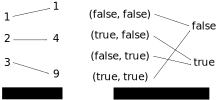
\includegraphics[width=0.8\textwidth]{./svg/function-as-arrows}
    \caption{Darstellung von Funktionen als Pfeildiagramm}
    \label{fig:FunAsArrows}
\end{figure}

Für diese Vorlesung beschränken wir uns auf Funktionen zwischen reellen Zahlen. Hier unterscheiden wir zwei Arten, je nachdem, ob der Funktionswert nur von einer reellen Zahl oder von mehreren abhängt.

\begin{definition}{Einstellige Funktion}{UnivarFun}
    Von einer \textbf{einstelligen reellwertigen Funktion} spricht man, wenn eine Abbildung $f: \R \to \R$ von einer reellen Zahl zu einer anderen reellen Zahl vorliegt.
\end{definition}

\begin{definition}{Mehrstellige Funktion}{MultivarFun}
    Von einer \textbf{$n$-stelligen reellwertigen Funktion} spricht man, wenn eine Abbildung $f: \R^n \to \R$ von einer Tupel reeller Zahlen zu einer anderen reellen Zahl vorliegt.
\end{definition}

Der Gewinn beim Verkauf eines Produkts in Abhängigkeit der produzierten Stückzahl stellt ein Beispiel für eine einstellige Funktion dar und könnte etwa $f: x \mapsto 0.2\text{Euro} \cdot x - 200\text{Euro}$ lauten (20 Cent Gewinn pro verkauften Produkt, 200  Fixkosten für Miete). Der elektrische Widerstand eines Drahtes in Abhängigkeit seiner Länge, seiner Querschnittsfläche und seines Materials wird dargestellt durch eine dreistellige Funktion und lautet $R: (l, A, \rho) \mapsto \rho \frac{l}{A}$.

Nun ist es für das praktische Rechnen auch erforderlich, Funktionen aufzuschreiben. Mathematisch lassen sich Funktionen in verschiedenen Formen als Gleichung angeben:

\begin{definition}{Explizite Form einer Funktion}{FunExplicit}
    Eine Funktion liegt in \textbf{expliziter Form} vor, wenn der Funktionswert als Rechenausdruck angegeben ist, der nur Variablen für die Argumente enthält.
\end{definition}

\begin{definition}{Implizite Form einer Funktion}{FunImplicit}
    Eine Funktion liegt in \textbf{impliziter Form} vor, wenn eine Beziehung (Gleichung) zwischen dem Funktionswert und den Argumenten angegeben ist.
\end{definition}

\begin{definition}{Parametrische Form einer einstelligen Funktion}{FunParam}
    Eine einstellige Funktion liegt in \textbf{Parameterdarstellung} vor, wenn sowohl das Argument als auch der Funktionswert jeweils als Funktion in Abhängigkeit eines Laufparameters $t$ angegeben sind:
    \begin{alignat*}{1}
      x &: t \mapsto u(t) \\
      y &: t \mapsto v(t)
    \end{alignat*}
    Hierdurch wird eine Funktion $f: x \mapsto v(u^{-1}(t))$ definiert. Voraussetzung dabei ist, dass $u$ umkehrbar sein muss.
\end{definition}

Je nach Anwendungsfall eignet sich eine Form besser als eine andere Form. Beispielsweise durch $f: x \mapsto x^2$ eine Funktion in expliziter Form gegeben. Formt man dies um zu $y-x^2=0$, erhält man eine mögliche implizite Form dieser Funktion. Ebenso ist $x^2+y^2=1$ eine implizite Form, welche eine Kreislinie beschreibt. Hierbei ist zu beachten, dass sich diese nicht global in explizite Form auflösen lässt, da zu den meisten Argumenten ein Funktionswert sowohl im oberen als auch im unteren Halbkreis existiert. Die Kreislinie lässt sich auch in parametrischer Form ausdrücken als $u(t) = \cos(t)$ und $v(t) = \sin(t)$ mit $t\in[0,2\pi)$.

\begin{figure}
    \centering
    \includegraphics[width=0.45\textwidth]{./gnuplot/implicit-fun-circle}
    \includegraphics[width=0.45\textwidth]{./gnuplot/implicit-fun-cross}
    \caption[Graphen impliziter Funktionen]{Graphen implizit gegebener Funktionen. Man beachte, dass immer nur ein Teil des Kreises und des Kreuzes als explizite Abbildung von Argumenten nach Funktionswerten aufgefasst werden kann.}
    \label{fig:ImplFun}
\end{figure}

Neben dem Pfeildiagramm gibt es noch weitere Möglichkeiten, ein- und mehrstellige Funktionen graphisch darzustellen.

\begin{definition}{Graph einer Funktion}{FunGraph}
    Der Graph $G$ einer n-stelligen Funktion $f: \R^n \to \R$ ist die Menge aller $(n+1)$-dimensionalen Punkte, die einem Argument-Funktionswerte-Paar entsprechen.

    $$
    G = \lbrace (p_1, p_2, ..., p_{n+1}) \in R^{n+1} | f((p_1, ..., p_n)) = p_{n+1} \rbrace
    $$

    Dieser Graph kann in einem $(n+1)$-dimensionalen kartesischen Koordinatensystem veranschaulicht werden.
\end{definition}

Ein kleiner Hinweis zum Zeichnen von Graphen. \href{http://www.gnuplot.info/}{gnuplot} ist ein Open-Source-Programm, mit dem man Graphen zeichnen kann, welches auch für die Illustrationen in diesem Skript verwendet wird. \href{http://maxima.sourceforge.net/}{Maxima} und \href{https://www.sagemath.org/}{sage} sind \mention{Cas}-Programme (Computer-Algebra-System), mit denen auch Graphen gezeichnet werden können. Online kann beispielsweise \href{https://www.geogebra.org/graphing}{GeoGebra} oder \href{https://www.wolframalpha.com/examples/mathematics/plotting-and-graphics/}{Wolfram Alpha} genutzt werden.

Für einstellige Funktionen ist der Graph zweidimensional und in einem $x-y$-Koordinatensystem wie in Abbildung \ref{fig:GraphUnivarFun} gut überschaubar. Für zweistellige Funktionen benötigt man bereits ein dreidimensionalen Koordinatensystem, in dem die Form des Graphen bereits schwerer zu überschauen ist, da der Graph meist auf eine zweidimensionale Bildschirmebene projiziert wird. Drei- und mehrstellige Funktionen sind auf diese Weise nur kaum bis gar nicht zur veranschaulichen. Die meisten Beispiele dieser Vorlesung werden sich daher auf ein- und zweidimensionale Funktionen beschränken. In Abbildung \ref{fig:GraphUnivarFun} ist der Graph einer einstelligen Funktion dargestellt. Abbildung \ref{fig:GraphMultivarFun} zeigt den Graph einer zweistelligen Funktion aus vier verschiedenen Blickwinkeln. Man beachte hierbei besonders die Seitensicht: Wird eines der beiden Argumente konstant gehalten und nur das anderen variiert, erhält man eine einstellige Funktion. Je nachdem, auf welchem Wert man das eine Argument konstant hält, ergeben sich verschiedene Funktionen.

\begin{figure}
    \centering
    \includegraphics[width=0.8\textwidth]{./gnuplot/example-univariate-function.png}
    \caption{Graph einer einstelligen Funktion}
    \label{fig:GraphUnivarFun}
\end{figure}

\begin{figure}
    \centering
    \includegraphics[width=0.45\textwidth]{./gnuplot/example-multivariate-function-1}
    \includegraphics[width=0.45\textwidth]{./gnuplot/example-multivariate-function-2}
    \includegraphics[width=0.45\textwidth]{./gnuplot/example-multivariate-function-3}
    \includegraphics[width=0.45\textwidth]{./gnuplot/example-multivariate-function-4}
    \caption{Graph einer zweistelligen Funktion}
    \label{fig:GraphMultivarFun}
\end{figure}

Für zweistellige Funktionen gibt es auch noch weitere Darstellungsformen, die manchmal übersichtlichen und einfacher zu erfassen sind. Die erste Darstellungsweise, die sogenannte \emph{Konturdarstellung}, wird etwa bei Wanderkarten für Abbildung zweidimensionaler Punkte der Erdoberfläche zur Höhe über Normalnull verwendet. Die Höhe an jedem Punkt wird farbig markiert, Kurven gleicher Höhe werden mit einer Linie dargestellt (Höhenlinien).

\begin{definition}{Konturlinie einer mehrstelligen Funktion}{ContLine}
    Unter einer \textbf{Konturlinie} zur Konstanten $c$ einer n-stelligen Funktion $f: \R^n\to\R$ versteht man die Menge $L_c$ aller Punkte des Definitionsbereichs, an dem der Funktionswert gleich der Konstanten $c$ ist.

    $$
       L_c = \lbrace x \in \R^n | f(x) = c \rbrace
    $$
\end{definition}

\begin{example}{Konturlinien einer Funktion}{ContLine}
    Gesucht sind die Konturlinien der zweistelligen Funktion $f: (x,y) \mapsto x^2+y^2$. Offensichtlich kann die Funktion keine negativen Werte annehmen. Wir bezeichnen die Konturlinienkonstante mit $R^2$. Nach Definition sind nun die Punkte $(x,y)\in\R^2$ gesucht, für die $x^2+y^2=R^2$ gilt. Unter Beachtung des Satzes von Pythagoras erkennen wir, dass es sich um alle Punkte handelt, deren Abstand zum Koordinatenursprung $R$ beträgt. Mithin handelt es sich bei den Konturlinien von $f$ also um zum Ursprung konzentrische Kreislinien. Diese sind in Abbildung \ref{fig:ExContLine} dargestellt.
\end{example}

\begin{figure}
    \centering
    \includegraphics[width=0.45\textwidth]{./gnuplot/example-contour-plot}
    \includegraphics[width=0.45\textwidth]{./gnuplot/example-pot-function}
    \caption[Konturlinien einer zweistelligen Funktion]{Konturlinien der Funktion $f(x,y)=x^2+y^2$ (links) und ihr Graph (rechts)}
    \label{fig:ExContLine}
\end{figure}

Ein Beispiel für die Konturlinien mit farbiger Hervorhebung für eine komplexere Funktion findet sich in Abbildung \ref{fig:ContourComplexFun}.

Als zweite Darstellungsform gibt es noch das sogenannte Gradientenfeld, wobei durch Pfeile angezeigt wird, in welcher Richtung die Funktionswerte am stärksten zunehmen. Dies ist etwa bekannt aus Wetterkarten, wo die Windrichtung (näherungsweise) als Gradient des Luftdruckes eingezeichnet ist.

\begin{definition}{Richtungsfeld einer mehrstelligen Funktion}{GradField}
    Unter dem \textbf{Richtungsfeld} (Gradientenfeld) einer $n$-stelligen Funktion $f: \R^n \to  \R$ versteht man die Funktion $G_f: \R^n \to \R^n$, welche jedem Punkt $\vec{r}=(x_1,x_2,...,x_n)$ des Definitionsbereichs von $f$ eine Richtung (einen $n$-dimensionalen Vektor) zuordnet, welcher in Richtung des stärksten Anstiegs von $f$ im Punkt $\vec{r}$ zeigt.
\end{definition}

Mathematisch entspricht das Richtungsfeld dem Gradienten $\grad{f}$ der Funktion. Wie genau dieser berechnet wird, lernen wir im nächsten Kapitel kennen. 

In Abbildung \ref{fig:ExGradField} ist das Richtungsfeld für die Funktion $f(x,y) = 1-x^2-y^2$ eingezeichnet. Die Richtung des stärksten Anstiegs verläuft immer radial in Richtung zum Koordinatenursprung. Aus der Anschauung ist dies unmittelbar klar, bei dem Graphen von $f$ handelt es sich um einen nach oben geöffnete Kesselform beziehungsweise einen "Berggipfel".

\begin{figure}
    \centering
    \includegraphics[width=0.35\textwidth]{./gnuplot/example-gradient-field}
    \includegraphics[width=0.55\textwidth]{./gnuplot/example-hill-function}
    \caption[Gradientenfeld einer zweistelligen Funktion]{Gradientenfeld der Funktion $f(x,y) = 1-x^2-y^2$ (links) und ihr Graph (rechts).}
    \label{fig:ExGradField}
\end{figure}

An dieser Stelle noch eine kurze Anmerkung zum sogenannten \emph{Feld}. Speziell in der Physik bezeichnet man mit einem Feld eine Größe, welche an jedem Punkt des Raums einen anderen Wert haben kann. Diese stellen mehrstellige Funktionen dar. Etwa ist der Luftdruck ein Feld, wo jedem Raumpunkt ein Luftdruckwert zugeordnet wird. Da der Luftdruck nur ein einzelne Zahl (=Skalar) ist, nennt man solche Felder auch skalare Felder. Das elektrische Feld ist ein vektorielles Feld und weist jedem Raumpunkt einen Vektor (Richtung und Betrag) zu, der angibt, welche Kraft eine geladene Masse an diesem Raumpunkt erfährt.

\section{Transformation von Funktionen}

Hat man Funktionen gegeben, kann man aus diesen neue Funktionen gewinnen, indem man diese geeignet kombiniert.

Zum Einen lassen sich zwei Funktionen $f$ und $g$ verketten, indem man sie hintereinander ausführt.

\begin{definition}{Komposition von Funktionen}{CompFun}
    Seien $f: B \to C$ und $g: A \to B$ zwei Funktionen mit den Rechenvorschriften $f: x \mapsto u(x)$ und $g: x \mapsto v(x)$. Die durch $h = f \circ g: A \to C$ definierte Funktion heißt \textbf{Komposition} (\emph{Verkettung}) von $f$ mit $g$ und ist gegeben durch:
    $$
        h: x \mapsto u(v(x))
    $$
    $f$ heißt dabei äußere Funktion und $g$ innere Funktion.
\end{definition}

\begin{example}{Verkettete Funktionen}{CompFun}
    Die Verkettung $f \circ g$ der Funktionen $f: x \mapsto -x$ und $g: x \mapsto x-3$ lautet $x \mapsto -(x-3) = 3-x$. Man beachte hierbei, dass beide Vorzeichen umgedreht werden. Zudem ist die Reihenfolge der Verkettung wichtig. Vertauscht man die Operanden, erhält man die verkettete Funktion $g \circ f: x \mapsto -x-3$.

    Die Funktion $f: x \to \sin(x^2)$ lässt sich darstellen als verkette Funktion, indem man für die innere Funktion $v(x) = x^2$ wählt und für die äußere Funktion $u(x) = \sin(x)$. Damit gilt $\sin(x^2) = u(v(x)) = u(x^2) = \sin(v(x))$.
\end{example}

Zum Zweiten kann man den Graphen einstelliger Funktionen entlang der Abszisse oder der Ordinate verschieben und stauchen. Diesen geometrischen Transformationen lassen sich durch einfache Modifikation an der Rechenvorschrift der Funktion erreichen und sind in Tabelle  \ref{lst:TranslateScaleFun} zusammengefasst und in Abbildung \ref{fig:TransformFunTrans} sowie \ref{fig:TransformFunScale} graphisch veranschaulicht.

\begin{listing}
    \begin{center}
        \begin{tabular}{ c | c | c }
            - & \textbf{x-Achse} & \textbf{y-Achse} \\
            \hline
            \textbf{Verschiebung} & \makecell{$f(x+c)$: nach links \\ $f(x-c)$: nach rechts} & \makecell{$f(x)+c$: nach oben \\ $f(x)-c$: nach unten} \\
            \hline
            \textbf{Skalierung} & \makecell{$f(a \cdot x)$ \\ $|a| > 1$: Stauchen \\ $|a| < 1$: Strecken \\ Für $a<0$ findet zusätzlich \\ Spiegelung an der y-Achse statt.} & \makecell{$a \cdot f(x)$ \\ $|a| > 1$: Strecken \\ $|a| < 1$: Stauchen \\ Für $a<0$ findet zusätzlich \\ Spiegelung an der x-Achse statt.}
        \end{tabular}
    \end{center}
    \caption[Verschiebung und Skalierung einer Funktion]{Verschiebung und Skalierung einer Funktion durch Modifikation der Funktionsgleichung}
    \label{lst:TranslateScaleFun}
\end{listing}

Die Skalierung erfolgt dabei immer bezüglich des Koordinatenursprungs. Bei solchen Transformationen einer Funktion ist unbedingt auf die Reihenfolge der Operationen zu achten. Es ist beispielsweise ein Unterschied, ob eine Funktion erst mit dem Faktor $2$ gestreckt wird und dann um $2$ nach rechts verschoben wird; oder erst verschoben und dann gestreckt wird, siehe auch Abbildung \ref{fig:TransformOrder}.

\begin{example}{Transformation von Funktionen durch Verschiebung und Skalierung}{TransformFunTranslScale}
    \begin{itemize}
        \item Die Funktion $x \mapsto (x-2)^2+3$ ist gegenüber $x \mapsto x^2$ um $2$ Einheiten nach rechts und um $3$ Einheiten nach oben verschoben. Der Scheitelpunkt liegt daher bei $(2,3)$.
        \item Die Funktion $x \mapsto 3\sin(2x)$ ist gegenüber $x \mapsto \sin(x)$ skaliert. Entlang der x-Achse ist mit dem Faktor $2$ gestaucht und hat daher die Periode $\frac{1}{2}\cdot 2\pi = \pi$. Entlang der y-Achse ist sie mit dem Faktor $3$ gestreckt und hat daher die Amplitude $3$.
        \item Wir betrachten die Funktion mit der Gleichung $f(x)$. Verschieben wir diese entlang der x-Achse um $c$ Einheiten, erhalten wir $g(x) = f(x-c)$. Skalieren wir weiterhin die so entstandene Funktion $g$ mit dem Faktor $a$ entlang der x-Achse, erhalten wir $h(x) = g(ax) = f(ax-c)$.
        \item Wenn wir andererseits zuerst entlang der x-Achse skalieren, erhalten wir $g(x) = f(ax)$. Nach Verschiebung entlang der x-Achse erhalten wir $h(x) = g(x-c) = f(a(x-c)) = f(ax-ac)$.
    \end{itemize}
\end{example}

Aus den letzten beiden Beispielen leitet sich die folgende Aussage ab:

\begin{statement}{Hintereinanderausführung von Verschiebung und Skalierung}{CombTranslScale}
    Sei $f$ eine einstellige Funktion und seien $a,c\in\R$ Konstanten. Dann ist
    \begin{enumerate}
        \item die Funktion $f(ax-c)$ gegenüber $f$ zuerst an der x-Achse um $c$ verschoben und dann entlang der x-Achse mit dem Faktor $a$ skaliert.
        \item die Funktion $f(a(x-c))$ gegenüber $f$ zuerst entlang der x-Achse mit dem Faktor $a$ skaliert und dann an der x-Achse um $c$ verschoben .
    \end{enumerate}
\end{statement}

\begin{figure}
    \centering
    \includegraphics[width=0.45\textwidth]{./gnuplot/transform-fun-translate}
    \caption{Verschiebung einer Funktion entlang der x- und y-Achse}
    \label{fig:TransformFunTrans}
\end{figure}

\begin{figure}
    \centering
    \includegraphics[width=0.45\textwidth]{./gnuplot/transform-fun-scale-x}
    \includegraphics[width=0.45\textwidth]{./gnuplot/transform-fun-scale-y}
    \caption{Skalierung einer Funktion entlang der x- und y-Achse}
    \label{fig:TransformFunScale}
\end{figure}

\begin{figure}
    \centering
    \includegraphics[width=0.65\textwidth]{./gnuplot/transform-translate-scale-order}
    \caption[Verschiebung und Skalierung in unterschiedlicher Reihenfolge]{Abhängigkeit der Reihenfolge von Verschiebung und Skalierung erhält man unterschiedliche Funktionen.}
    \label{fig:TransformOrder}
\end{figure}



\section{Eigenschaften von Funktionen}

Bisher haben wir Funktionen nur als allgemeine Zuordnung von Elemente einer Menge zu Elementen einer anderen Menge kennengelernt. In der Analyse von und bei der Arbeit mit Funktionen ist es wichtig zu wissen, welche Eigenschaften eine Funktion hat. Im Folgenden werden einige besonders wichtige Eigenschaften von Funktionen besprochen.

\subsection{Umkehrbarkeit}

Mittels einer Funktionsgleichung lässt sich berechnen, welcher Funktionswert zu einem Argument gehört. Für die Praxis ist es oft auch relevant, zu einem gegebenen Funktionswert das zugehörige Argument zu berechnen. In der Analyse von radioaktiven Zerfällen kann man sich etwa fragen, wie lange man warten muss, bis die Strahlungsdosis auf die Hälfte oder auf ein Drittel abgefallen ist. Mathematisch entspricht dies der Umkehrfunktion, welche eine Abbildung von den Funktionswerten zu den Argumenten vermittelt. Nun ist es so, dass nicht jede Funktion umkehrbar ist. Um beschreiben zu können, wann dies möglich ist, müssen wir zuerst die Begriffe \emph{Injektivität} und \emph{Surjektivität} einer Funktion definieren. Dies werden wir allgemeingültig für alle Funktionen tun, nicht nur für reellwertige oder einstellige Funktionen.

\begin{definition}{Injektivität einer Funktion}{Injective}
    Sei $f: \mathbb{D} \to \mathbb{C}$ eine Funktion mit Definitionsbereich $\mathbb{D}$ und Wertebereich $\mathbb{C}$. $f$ heißt \textbf{injektiv}, wenn eine Funktion $g: \mathbb{C} \to \mathbb{D}$ existiert mit der Eigenschaft:
    $$
    g \circ f = \mathbbm{1}_\mathbb{D}
    $$
    Äquivalent dazu ist die Forderung, dass kein Funktionswert doppelt angenommen wird, sich also gleiche Funktionswerte nur aus gleichen Argumenten ergeben: $\forall x_1,x_2\in\mathbb{D}: f(x_1)=f(x_2) \implies x_1=x_2$.
\end{definition}

\begin{definition}{Surjektivität einer Funktion}{Surjective}
    Sei $f: \mathbb{D} \to \mathbb{C}$ eine Funktion mit Definitionsbereich $\mathbb{D}$ und Wertebereich $\mathbb{C}$. $f$ heißt \textbf{surjektiv}, wenn eine Funktion $g: \mathbb{C} \to \mathbb{D}$ existiert mit der Eigenschaft:
    $$
    f \circ g = \mathbbm{1}_\mathbb{C}
    $$
    Äquivalent dazu ist die Forderung, dass jeder Funktionswert wenigstens einem Argument zugeordnet ist, dass also $f(\mathbb{D}) = \mathbb{C}$ gilt. Dabei bezeichnet $f(\mathbb{D})$ die Menge aller Elemente, die man erhält wenn man auf jedes Argument die Funktion anwendet.
\end{definition}

Anhand dieser beiden Definitionen können wir nun ein Kriterium dafür angeben, wann die Umkehrfunktion zu einer Funktion existiert.

\begin{statement}{Umkehrbarkeit einer Funktion}{InverseFun}
    Sei $f: \mathbb{D} \to \mathbb{C}$ eine Funktion mit Definitionsbereich $\mathbb{D}$ und Wertebereich $\mathbb{C}$. $f$ heißt \textbf{bijektiv}, wenn $f$ sowohl injektiv als auch surjektiv ist. Dann existiert genau eine Funktion $f^{-1}: \mathbb{C} \to \mathbb{D}$, welche die Bedingungen für Injektivität und Surjektivität erfüllt:
    $$
    f^{-1} \circ f = \mathbbm{1}_\mathbb{D}, f \circ f^{-1} = \mathbbm{1}_\mathbb{C}
    $$
    Es heißt dann $f^{-1}$ die \textbf{Umkehrfunktion} zu $f$.
\end{statement}

Bezüglich der Notation beachte man, dass $f^{-1}$ nicht das Reziproke $\frac{1}{f}$ bezeichnet, sondern nur eine symbolische Schreibweise für die Umkehrfunktion ist. Sie leitet sich darauf ab, dass die Hyperbelfunktion $x \mapsto 1/x$ die Umkehrfunktion zur linearen Funktion $x \mapsto x$ ist.

Rechnerisch erhält man die Umkehrfunktion aus der Funktionsgleichung $y = f(x)$, indem man diese nach $x = f^{-1}(y)$ umstellt. Man vertauscht dabei also $x$ und $y$. Graphisch entspricht das Bilden der Umkehrfunktion der Spiegelung an der Hauptgeraden $y=x$.

\begin{figure}
    \centering
    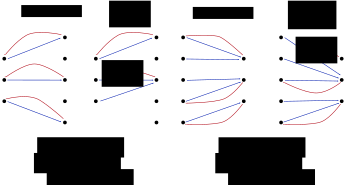
\includegraphics[width=0.95\textwidth]{./svg/injective-surjective}
    \caption[Injektivität und Surjektivität]{Visuelle Darstellung der Definition von Injektivität und Surjektivität. Es ist jeweils eine Beispiel für eine Abbildung dargestellt, welche die Bedingung erfüllt, und ein Beispiel, wo sie die Bedingung nicht erfüllt. Die Bedingung, dass sich die Identitätsfunktion ergeben soll, bedeutet graphisch, dass man an einem Punkt anfängt, den Pfeilen folgt, und schließlich wieder am Ausgangspunkt ankommt. Das ist bei dem nicht-injektiven beziehungsweise nicht-surjektiven Beispiel nicht möglich.}
    \label{fig:InjectSurject}
\end{figure}

\begin{figure}
    \centering
    \includegraphics[width=0.5\textwidth]{./gnuplot/inverse-function-reflection}
    \caption[Graphische Bedeutung der Umkehrfunktion]{Graphische Bedeutung der Umkehrfunktion. Man erhält die Umkehrfunktion $\ln(x)$ durch Spiegelung der Funktion $e^x$ an der Hauptdiagonalen $y=x$.}
    \label{fig:InvFunRefl}
\end{figure}

\begin{example}{Untersuchung einer Funktion auf Umkehrbarkeit}{}
    \begin{enumerate}
        \item Die Funktion $f: (-\infty,\infty) \to (-\infty,\infty)$ mit $x \mapsto x^2$ ist nicht surjektiv, denn es kann keine Abbildung $g: (-\infty,\infty) \to (-\infty,\infty)$ geben. Für diese müsste etwa auch $(f \circ g)(-1) = g(-1)^2 = -1$ gelten, was aber nicht möglich ist, da bei der Quadratbildung nur nichtnegative Werte möglich sind. Durch Einschränkung des Wertebereichs kann dieses Problem wie im nächsten Beispiel illustriert gelöst werden.
        \item Die Funktion $f: (-\infty,\infty) \to [0,\infty)$ mit $x \mapsto x^2$ ist surjektiv, aber nicht injektiv. Sie ist surjektiv, da etwa die Funktion $g: [0,\infty) \to (-\infty,\infty)$ mit $x \mapsto \sqrt{x}$ existiert,  sodass gilt $(f \circ g)(x) = (\sqrt{x})^2 = x$. Die Funktion ist nicht eindeutig, genauso hätten wir $g: x \mapsto -\sqrt{x}$ wählen können, auch hier gilt $(-\sqrt{x})^2 = x$. Allerdings ist $f$ nicht injektiv, für beide Kandidaten einer Umkehrfunktion ist $(g \circ f)(x) = \pm\sqrt{x^2} = \pm|x| \ne x$. Durch Einschränkung des Definitionsbereichs auch wie im nächsten Beispiel auch dieses Problem umgangen werden.
        \item Die Funktion $f: (0,\infty) \to [0,\infty)$ mit $x \mapsto x^2$ ist injektiv. Es existiert die Funktion $g: x \mapsto \sqrt{x}$, sodass gilt: $\sqrt{x^2}=|x|=x$ (da $x\ge 0$). Zudem gilt auch $\left(\sqrt{x}\right)^2=x$, $f$ ist also surjektiv. Mithin ist $f$ bijektiv, es existiert die Umkehrfunktion $f^{-1}(x) = \sqrt{x}$, welche den rechten Parabelast darstellt.
        \item Die Funktion $f: (-\infty,0] \to [0,\infty)$ mit $x \mapsto x^2$ ist ebenso umkehrbar. Es existiert die Funktion $g: x \mapsto -\sqrt{x}$, sodass gilt: $-\sqrt{x^2}=-|x|=x$ (da $x\le 0$). Die Umkehrfunktion lautet $f^{-1}(x) = -\sqrt{x}$, welche den linken Parabelast darstellt.
        \item Die Funktion $f: (-\infty,\infty) \to (0, \infty)$ mit $x \mapsto e^x$ ist umkehrbar. Die Funktion $f^{-1}: (0, \infty) \to (-\infty,\infty)$ mit $x \mapsto \ln(x)$ erfüllt die Eigenschaften für die Injektivität und die Surjektivität, da gilt: $e^{\ln(x)} = \ln(e^x) = x$.  Mithin ist $\ln(x)$ die Umkehrfunktion zu $e^x$.
    \end{enumerate}
\end{example}

\subsection{Monotonie}

Eine Funktion kann auch daraufhin untersucht werden, ob ihr Graph beständig ansteigt oder abfällt. Wir wollen uns hier auf einstellige Funktionen beschränken, für mehrstellige Funktionen kann es passieren, dass die Funktionswerte in eine Richtung fallen und in einer anderen Richtung steigen.

\begin{definition}{Monotonie einer einstelligen Funktionen}{UnivarMonotonic}
    Eine einstellige, reellwertige Funktion $f: \R \to \R$ heißt in einem offenen Interval $U\subset\R$ \textbf{monoton steigend} (\textbf{fallend}), wenn größere Argumente immer gleiche oder größere (kleinere) Funktionswerte zur Folge haben, falls also gilt:
    $$
        \forall x_1,x_2 \in U: x_2 > x_1 \implies f(x_2) \ge f(x_1)
    $$
    $$
      ( \forall x_1,x_2 \in U: x_2 > x_1 \implies f(x_2) \le f(x_1) )
    $$
    Gilt auf der rechten Seite der Implikation sogar einer Größer-Zeichen (Kleiner-Zeichen), heißt die Funktion \textbf{streng monoton steigend} (\textbf{streng monoton fallend}).
\end{definition}

Wenn eine Funktion auf ihrem gesamten Definitionsbereich monoton ist, heißt sie monoton steigende oder fallende Funktion. Ansonsten unterteilt man den Definitionsbereich in Teilmengen und untersucht dort auf Monotonie.

\begin{example}{Untersuchung auf Monotonie}{ExamMonot}
    \begin{enumerate}
        \item Die lineare Funktion $x \mapsto 3x$ ist streng monoton steigend, denn aus $x_2 > x_1$ folgt $3x_2^2 > 3x_1^2$.
        \item Die quadratische Funktion $x \mapsto x^2$ ist nur auf Teilbereichen monoton. Für $x\le 0$ ist sie streng monoton fallend, denn aus $x_2 > x_1$ folgt für negative Werte $x_2^2 < x_1^2$. Analog ist sie für $x\ge 0$ streng monoton steigend.
        \item Die Sinusfunktion $x \mapsto \sin(x)$ ist $x\in[\degrees{0},\degrees{90}]$ streng monoton steigend, für $x\in[\degrees{90}, \degrees{0},270]$ streng monoton fallend und für $x\in[\degrees{270},\degrees{360}]$ wieder streng monoton steigend.
        \item Die konstante Funktion $x \mapsto 42$ ist sowohl monoton steigend als auch monoton fallend, aber nicht streng monoton steigend oder fallend.
    \end{enumerate}
\end{example}

\subsection{Symmetrie}

Ein weiteres wichtiges Merkmal einer Funktion ist ihr sogenanntes Symmetrieverhalten. Dieses gibt an, wie sich der Funktionswert ändert, wenn das Argument negiert wird, also beispielsweise $-3$ statt $3$ in die Funktionsgleichung eingesetzt wird. Man unterscheidet zwei wesentliche Fälle:

\begin{definition}{Symmetrie einer einstelligen Funktionen}{UnivarSymm}
    Sei $f: \R \to \R$ eine einstellige, reellwertige Funktion.

    $f$ heißt \textbf{achsensymmetrisch} oder \textbf{gerade} Funktion, wenn ihr Funktionswert sich unter Negation des Arguments nicht ändern, falls also für alle Argumente gilt: $f(x) = f(-x)$.

    $f$ heißt \textbf{punktsymmetrisch} oder \textbf{ungerade} Funktion, wenn ihr Funktionswert sich unter Negation des Arguments ebenfalls negiert, aber betragsmäßig gleich bleibt, falls also für alle Argumente gilt: $f(x) = -f(-x)$.
\end{definition}

Man beachte hierbei, dass die Wahl der Begriffe \emph{achsensymmetrisch} und \emph{punktsymmetrisch} nicht willkürlich gewählt sind. Man überlegt sich schnell, dass achsensymmetrische Funktionen tatsächlich symmetrisch bezüglich der vertikalen Spiegelachse $x=0$ sind. Ebenso sind punktsymmetrische Funktionen punktsymmetrisch zum Punkt $(0,0)$.

\begin{example}{Untersuchung auf Symmetrie}{ExamSymm}
    \begin{itemize}
        \item Die Funktion $x \mapsto x^2$ ist eine gerade Funktion, denn es gilt $f(-x) = (-x)^2 = (-1)^2 x^2 = x^2 = f(x)$.
        \item Die Funktion $x \mapsto x^3$ ist eine ungerade Funktion, denn es gilt $f(-x) = (-x)^3 = (-1)^3 x^3 = -x^3 = -f(x)$.
    \end{itemize}
\end{example}

\begin{figure}
    \centering
    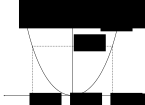
\includegraphics[width=0.45\textwidth]{./svg/axis-symmetric-fun}
    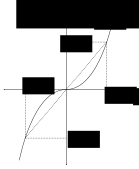
\includegraphics[width=0.45\textwidth]{./svg/point-symmetric-fun}
    \caption[Gerade und ungerade Funktionen]{Links: Achsensymmetrische Funktion. Der rechte Teile der Parabel geht unter Spiegelung an der Ordinate in den linken Teil über. Rechts: Punktsymmetrische Funktion: Der rechte Teil der kubischen Parabel geht unter Punktspiegelung am Ursprung in den linken Teil über.}
    \label{fig:ExAxisSymFun}
\end{figure}

Von besonderer Bedeutung sind diese beiden Symmetrieeigenschaften, da sich alle Funktionen, sofern sie denn für positive und negative Argumente überhaupt definiert sind, zerlegen lassen in die Summe aus einem geraden und einem ungerade Anteil.

\begin{statement}{Gerader und ungerader Anteil einer Funktion}{SplitEvenOddFun}
    Sei $f: \R \to \R$ eine einstellige reellwertige Funktion mit einem Definitionsbereich $\mathbb{D}$ derart, dass $x\in\mathbb{D} \iff -x\in\mathbb{D}$ gilt, also zu jedem Argument auch sein Negiertes zum Definitionsbereich gehört. Seien weiterhin $e$ und $o$ wie folgt definierte Funktionen:

    \begin{alignat*}{1}
        e(x) &= \frac{f(x) + f(-x)}{2} \\
        o(x) &= \frac{f(x) - f(-x)}{2}
    \end{alignat*}

    Dann ist $e$ eine gerade (\emph{even}) Funktion und $o$ eine ungerade (\emph{odd}) Funktion; und es gilt: $f(x) = e(x) + o(x)$.
\end{statement}

Dass die Funktionen $e$ und $o$ gerade beziehungsweise ungerade sind, zeigt man leicht anhand der Definition. Durch Aufaddieren beider Funktionen und Zusammenfassen des Bruches zeigt man, dass man so die ursprüngliche Funktion $f$ erhält. Dieser Zerlegung kommt unter anderem deswegen Bedeutung zu, weil sie eine Definition der trigonometrischen und hyperbolischen Funktionen über die Exponentialfunktion erlaubt, wie wir im nächsten Abschnitt zu speziellen Funktionen sehen werden.

\begin{example}{Ermittlung des geraden und ungeraden Anteils einer Funktion}{CompEvenOddPart}
    Gesucht ist der gerade und ungerade Anteil von $x \mapsto x^2+x^3$. Nach Aussage \ref{stmt:SplitEvenOddFun} berechnen wir $e(x) = \frac{(x^2+x^3)+((-x)^2)+(-x)^3)}{2} = \frac{x^2+x^3+x^2-x^3}{2} = x^2$ und $o(x) = \frac{(x^2+x^3)-((-x)^2)+(-x)^3)}{2} = \frac{x^2+x^3-x^2+x^3}{2} = x^3$. Dies ist deshalb nicht überraschend, da wir bereits wissen, dass $x\mapsto x^2$ gerade und $x \mapsto x^3$ ungerade ist.
\end{example}

\subsection{Periodizität}

Die Periodizität ist eine Eigenschaft von periodischen Funktionen, deren Funktionswerte sich nach einer bestimmten Periode immer wiederholen. Die Sinus- und Kosinusfunktionen sind ein bekanntes Beispiel für periodische Funktionen.

\begin{definition}{Periode einer einstelligen Funktion}{PeriodUnivarFun}
    Sei $f: \R \to \R$ eine einstellige reellwertige Funktion mit Definitionsbereich $\mathbb{D}$. $f$ heißt \textbf{periodisch}, wenn es eine reelle Zahl $p>0$ derart gibt, dass gilt:
    $$
        \forall x \in \mathbb{D}: f(x) = f(x+p)
    $$
    Jede solche Zahl $p$ heißt dann \textbf{Periode}. Die kleinste solche Zahl $p$ nennt man \textbf{primitive Periode} der Funktion.
\end{definition}

Aus dieser Definition erkennt man sofort, dass wenn $p$ eine Periode der Funktion ist, auch $2p$ eine Periode ist: per Definition gilt $f(x) = f(x+p)$ und $f(x+p)=f(x+p+p)=f(x+2p)$, mithin also auch $f(x) = f(x+2p)$. Allgemein ist jedes ganzzahlige Vielfache der primitiven Periode auch eine Periode. Oft wird statt dem Begriff \emph{primitive Periode} auch einfach nur \emph{Periode} verwendet.

\begin{example}{Untersuchung der Periodizität}{ExamPeriod}
    \begin{enumerate}
        \item Die Funktion $x \mapsto \tan(x)$ ist periodisch, denn beispielsweise ist $p=2\pi$ eine Periode, da $\tan(x+2\pi)=\frac{\sin(x+2\pi)}{\cos(x+2\pi)} = \frac{\sin(x)}{\cos(x)} = \tan(x)$ gilt. Die kleinste Periode ist $p=\pi$ (=$\degrees{180}$) und stell damit die primitive Periode der Tangensfunktion dar.
        \item Auch die konstante Funktion $x \mapsto 42$ ist periodisch. Jedes $p>0$ ist eine Periode der Funktion. Allerdings gibt es keine kleinste Periode (da $p=0$ per Definition ausgeschlossen ist).
    \end{enumerate}
\end{example}

\subsection{Stetigkeit}

In der Analysis wollen wir Funktionen mittels der Infinitesimalrechnung analysieren. Eine wesentliche Voraussetzung dafür ist, dass eine Funktion ausreichend "glatt" verläuft und ihre Funktionswerte nicht plötzlich springen. Graphisch kann man sich dies so vorstellen, dass man den Graphen der Funktion zeichnen kann, ohne den Stift absetzen zu müssen. Diese Eigenschaft, welche eine solche Funktionen erfüllen muss, nennt man die \emph{Stetigkeit}. Um diese mathematisch fassen zu können, benötigen wir erneut den Begriff der Grenzwertbildung für mehrstellige Funktonen, den wir bereits in \ref{def:LimFun} kennengelernt haben.

\begin{definition}{Stetigkeit einer reellwertigen Funktion}{ContFun}
    Sei $f: \R^n \to \R$ eine $n$-stellige, reellwertige Funktion mit Definitionsbereich $\mathbb{D}$. $f$ heißt \textbf{stetig} an der Stelle $x_0\in\mathbb{D}$, wenn der Grenzwert für diese Stelle existiert und dem dem Funktionswert gleich ist, also gilt:
    $$
        \lim\limits_{x_0\to x} f(x) = f(x_0)
    $$
    Falls $f$ für alle Werte des Definitionsbereichs stetig ist, heißt $f$ eine \textbf{stetige Funktion}.
\end{definition}

Im engen Zusammenhang mit der Stetigkeit steht die sogenannte stetige Ergänzung einer Funktion. Manche Funktionen sind aufgrund ihrer Struktur (Quotient) für einen einzelne Stelle (Definitionslücke) nicht erklärt. Dennoch kann es vorkommen, dass die Funktionen für alle Argumente in der Nähe der Definitionslücke Funktionswerte besitzt, die nahe beieinander liegen. Man kann dann die Definitionslücke schließen, in dem man als Funktionswert für diese Stelle den Grenzwert nimmt.

\begin{definition}{Stetige Ergänzung einer Funktion}{ContinousContinuation}
    Sei $f: \R^n\to\R$ eine mehrstellige Funktion mit Definitionsbereich $\mathbb{D}\subseteq\R^n$ und $x_0\notin\mathbb{D}$ eine Stelle außerhalb des Definitionsbereichs (\textbf{Definitionslücke}). Falls der Grenzwert $\lim\limits_{x\to x_0} = \alpha$ existiert, heißt die Funktion $\bar{f}$, welche durch Hinzunahme des Grenzwert aus $f$ entsteht, die \textbf{stetige Ergänzung} von $f$:
    $$
        \bar{f}: x \to \begin{cases}
            f(x) & , x \in \mathbb{D} \\
            \alpha & , x = x_0
        \end{cases}
    $$
    $\bar{f}$ hat somit nun den Definitionsbereich $\mathbb{D} \cup \lbrace x_0 \rbrace$.
\end{definition}

\begin{example}{Untersuchen der Stetigkeit einstelliger Funktionen}{ExamContUnivarFun}
    \begin{itemize}
        \item Die meisten aus der Schulmathematik, bekannten Funktion sind im jeweiligen Definitionsbereich stetig. Dazu gehören lineare Funktion, quadratische Funktionen, Potenz-, Exponential-, und Logarithmusfunktionen sowie trigonometrische Funktionen.
        \item Die Funktion $x\mapsto 1/x$ ist nicht stetig in $x_0=0$, da für diese Stelle gar kein Funktionswert erklärt ist. Zudem ist sie auch nicht stetig ergänzbar, da der Grenzwert $\lim\limits_{x\to 0}$ nicht existiert.
        \item Die Funktion $x \mapsto \frac{\sin(x)}{x}$ ist nicht stetig in $x_0=0$, da für diese Stelle ebenfalls keine Funktionswert erklärt ist. Allerdings ist sie stetig ergänzbar, denn mit der Regel von L'Hôpital folgt $\lim\limits{x\to 0} \frac{\sin(x)}{x} = \lim\limits{x\to 0} \frac{\cos(x)}{1} = 1$. Die durch $\bar{f} = \begin{cases} \sin(x)/x & , x \ne 0 \\ 1 & , x = 0 \end{cases}$ erklärte Funktion ist die (nun auf ganz $\R$ erklärte) stetige Ergänzung von $f$.
        \item Die sogenannte Signum-Funktion (Vorzeichenfunktion) $\text{sgn}: x \to \begin{cases} -1 &, x < 0 \\ 0 &, x = 0 \\ 1 &, \ge 0 \end{cases}$ ist nicht stetig in $x_0=0$. Während zwar ein Funktionswert an der Stelle existiert, existiert der Grenzwert nicht, da der linksseitige Grenzwert $\lim\limits_{x\to 0^-} \text{sgn}(x) = -1$ beträgt, während der rechtsseitige Grenzwert $\lim\limits_{x\to 0^+} \text{sgn}(x) = +1$ lautet.
    \end{itemize}
\end{example}

In Abbildung \ref{fig:NonContFun} sind zwei unstetige Funktionen abgebildet. Bei der Funktion links liegt eine Sprungstelle bei $0$ vor, da die Funktion dort plötzlich von einem Funktionswert zu einem anderen springt. Rechts liegt eine hebbare Definitionslücke vor, die durch stetige Ergänzung geschlossen werden kann.

\begin{figure}
    \centering
    \includegraphics[width=0.45\textwidth]{./gnuplot/example-non-continous-function-1}
    \includegraphics[width=0.45\textwidth]{./gnuplot/example-non-continous-function-2}
    \caption{Beispiele für unstetige Funktionen}
    \label{fig:NonContFun}
\end{figure}

\subsection{Spezielle Stellen}

Es gibt einige Punkte und Stellen von Funktionen, die von besonderem Interesse sind:

\begin{definition}{Besondere Stellen einer reellwertigen Funktion}{SpecValues}
    Sei $f: \R^n\to\R$ eine Funktion mit Definitionsbereich $\mathbb{D}$. Dann heißt
    \begin{itemize}
        \item $x_0\in\mathbb{D}$ eine \textbf{Nullstelle}, wenn gilt $f(x_0) = 0$.
        \item $(0, f(0))$ der \textbf{y-Achsenschnittpunkt}, falls $0$ zum Definitionsbereich gehört.
        \item $x_0 \in\mathbb{D}$ eine \textbf{hebbare Definitionslücke}, wenn $f$ stetig ist in $x_0$.
        \item $x_0 \in\mathbb{D}$ eine \textbf{Sprungstelle}, wenn $f$ nicht stetig ist in $x_0$.
        \item $x_0 \notin \mathbb{D}$ eine \textbf{Polstelle}, wenn der links- oder rechtsseitige Grenzwert bestimmt divergent ist.
    \end{itemize}
\end{definition}

Eine Nullstelle ist eine Stelle, wo der Funktionswert identisch $0$ ist. Rechnerisch ermittelt man Nullstellen, indem man die Rechenvorschrift für die Funktionswert gleich $0$ setzt und nach dem Argument umstellt. Der Frage, ob und welche Nullstellen eine Funktion hat, kommt besondere Bedeutung bei, da die Lösung von Gleichungen sich immer formulieren lässt als die Suche nach Nullstellen. Falls etwa $\sin(xy) = x+y$ gelöst werden soll, kann man dies auch formulieren als die Suche nach Nullstellen der zweistelligen Funktion $f: (x,y) \mapsto \sin(xy)-x-y$.

Eine Polstelle kann man sich vorstellen als eine vertikale Achse, an die sich der Graph der Funktion annähert. Ein Sprungstelle bedeutet graphisch, dass man dort den Stift absetzen muss, um den Graph zu zeichnen.

Ein Beispiel für eine hebbare Definitionslücke und eine Sprungstelle ist bereits in Abbildung \ref{fig:NonContFun} dargestellt. Abbildung \ref{fig:SpecValFun} zeigt graphisch die Bedeutung einer Nullstelle, einer Polstelle, und eines y-Achsen-Schnittpunkts.

\begin{example}{Nullstellen einer quadratischen Funktionen}{RootQuadFun}
    Sei $f: x \to ax^2 + bx +c$ eine quadratische Funktion mit $a,b,c\in\R$. Die Nullstellen ergeben sich durch Lösen der Gleichung $f(x) = 0$. Wir formen zuerst die Rechenvorschrift durch quadratische Ergänzung um: $ax^2 + bx +c = a\left(x + \frac{b}{a}x^2 + \frac{c}{a}\right) = a\left(\left(x+u\right)^2+v\right)$, wobei sich $u=\frac{b}{2a}$ ergibt und daraus dann $v=\frac{c}{a}-\left(\frac{b}{2a}\right)^2$. Somit müssen wir nun $a\left((x+\frac{b}{2a})^2+\frac{c}{a}-\left(\frac{b}{2a}\right)^2\right) = 0$ lösen. Es ergibt sich die Formel für die Lösung quadratischer Gleichungen:
    \begin{equation}
        x_{1,2} = -\frac{b}{2a} \pm \sqrt{\left(\frac{b}{2a}\right)^2 - \frac{c}{a}} \label{eq:RootQuadGen}
    \end{equation}
    Mit den Abkürzungen $p=\frac{b}{a}$ und $q=\frac{c}{a}$ folgt daraus die bekannte p-q-Formel:
    \begin{equation}
        x_{1,2} = -\frac{p}{2} \pm \sqrt{\frac{p^2}{4}-q} \label{eq:RootQuadSpec}
    \end{equation}
\end{example}

\begin{figure}
    \centering
    \includegraphics[width=0.6\textwidth]{./gnuplot/example-special-points}
    \caption[Nullstelle, y-Achsenschnittpunkt und Polstelle]{Beispiel einer Funktion mit Nullstelle, y-Achsenschnittpunkt und Polstelle}
    \label{fig:SpecValFun}
\end{figure}

\subsection{Extremwerte}

In der Praxis ist es oft von Bedeutung, herauszufinden, wann eine abhängige Größe ihren kleinsten oder größten Wert annimmt. Etwa will man die zu produzierende Stückzahl bestimmen, wo der zu erwartende Gewinn maximiert ist. Bei der Herstellung von Cola-Dosen will man diese so dimensionieren, dass das Verhältnis von Oberfläche zu Volumen besonders klein ist, damit man möglichst wenig Material verbraucht.

\begin{definition}{Extremstelle einer reellwertigen Funktion}{ExtrFun}
    Sei $f: \R^n \to \R$ eine $n$-stellige reellwertige Funktion. Eine Stelle $x_0\in\mathbb{D}$ heißt ein \textbf{globales Maximum} (\textbf{globales Minimum}) von $f$ bezüglich einer Menge $M\subset\mathbb{D}$, falls der Funktionswert an dieser Stelle kleiner oder gleich (größer oder gleich) aller Funktionswerte in $M$ ist:
    $$
		\forall x \in M: f(x) \le f(x_0)
	$$
	$$
		(\forall x \in M: f(x) \ge f(x_0))
	$$
    
    Falls es nur eine offene Umgebung $U_{x_0}\subset M$ um diese Stelle gibt, in der dies gilt, heißt $x_0$ ein \textbf{lokales Maximum} (\textbf{lokales Minimum}) bezüglich $M$:
    $$
        \forall x \in U_{x_0}: f(x) \le f(x_0)
    $$
    $$
        (\forall x \in U_{x_0}: f(x) \ge f(x_0))
    $$
\end{definition}

Diese Definition ist in Abbildung \ref{fig:ExtrValFun} veranschaulicht. Dort ist eine Funktion $f$ mit Definitionsbereich $\mathbb{D} = [-4.5, 4.5]$ dargestellt. Bei den Stellen \circled{1} und \circled{5} handelt es sich um globale Minima, denn im gesamten Definitionsbereich $[-4.5,4.5]$ gibt es keinen kleineren Funktionswert. Analog dazu handelt es sich bei den Stellen \circled{2} und \circled{4} um globale Maxima, denn im gesamten Definitionsbereich $[-4.5,4.5]$ gibt es keinen größeren Funktionswert. Die Stelle \circled{3} ist keine globale Extremstelle, denn im Definitionsbereich existieren sowohl kleinere als auch größere Funktionswerte. Allerdings handelt es sich um ein lokales Minimum, denn der Funktionswert ist etwa in der offenen Umgebung $(-1:1)$ der kleinste. Schließlich sind die mit \circled{x} markierten Stellen bei $x=\pm 2$ gar keine Extremstellen, denn in jeder noch so kleinen Umgebung um $2$ beziehungsweise $-2$ gibt es sowohl größere als auch kleinere Funktionswerte.

\begin{figure}
    \centering
    \includegraphics[width=0.45\textwidth]{./gnuplot/extreme-values-function}
    \caption{Lokale und globale Extremstellen einer Funktion}
    \label{fig:ExtrValFun}
\end{figure}

Eine wichtige Aussage über die Existenz von Extremstellen liefert der folgende Satz. Im nächsten Kapitel zur Infinitesimalrechnung werden wir noch Möglichkeiten kennenlernen, stetige Funktionen auf Extremstellen zu untersuchen.

\begin{statement}{Satz von Weierstraß}{WeierstrassExtrem}
    Jede stetige Funktion $f$ mit einem Definitionsbereich, der beschränkt und abgeschlossen ist, hat dort ein absolutes Maxima und ein absolutes Minima.
\end{statement}

Eine beschränkte Menge ist eine solche, in der es für den Abstand aller Paare von zwei Punkten eine endliche Obergrenze gibt. Abgeschlossen ist eine Menge, wenn sie einen Rand hat. Etwa sind alle abgeschlossenen Intervalle wie $[-3,5]$ oder $[-2,2]\times[-2,2]$ beschränkte Mengen.

\subsection{Verhalten im Unendlichen}

Manchmal ist es nicht von Interesse, wie sich eine Funktion für konkrete Werte verhält, sonder nur, was passiert, wenn man sehr große oder sehr kleine Werte einsetzt. Beispielsweise interessiert in der Informatik bei der Analyse von Algorithmen die sogenannte asymptotische Laufzeit oder der asymptotische Speicherverbrauch. Diese beschreiben, wie lange beziehungsweise wieviel Speicher ein Computerprogramm in Abhängigkeit der Größe der Eingabedaten benötigt.

\begin{definition}{Horizontale Asymptote einer einstelligen Funktion}{AsymptUnivar}
    Eine horizontale Asymptote $y=c$ einer Funktion $f: \R \to R$ liegt vor, wenn sich die Funktion der Zahl $c\in\R$ für große oder kleine Argumente annähert: $\lim\limits_{x\to\pm\infty} f(x) = c$.
\end{definition}

Oft ist es auch interessant zu betrachten, wie sich eine Funktion $f$ \emph{im Vergleich zu einer anderen} Funktion $g$ verhält. Man betrachtet dazu das Verhältnis $\frac{f(x)}{g(x)}$ und schaut, wie sich dieses Verhältnis für große Werte verhält.

\begin{definition}{Landau-Symbole}{LanSymb}
    Seien $f,g: \R \to \R$ zwei reellwertige Funktionen und $q(x) = \frac{f(x)}{g(x)}$ ihr Quotient. Dann heißt
    \begin{enumerate}
        \item $f \in \mathcal{O}(g)$, wenn der Quotient $q$ für große Werte endlich bleibt: $\lim\limits_{x\to\infty} |q(x)| < \infty$.
        \item $f \in o(g)$, wenn der Quotient $q$ für große Werte gegen $0$ strebt: $\lim\limits_{x\to\infty} |q(x)| = 0$.
        \item $f \sim g$, wenn der Quotient $q$ für große Werte gegen $1$ strebt: $\lim\limits_{x\to\infty} q(x) = 1$.
    \end{enumerate}
    Analog dazu kann man auch das Verhalten für $-\infty$ betrachten.
\end{definition}

Anschaulich bedeutet $f \in \mathcal{O}(g)$, dass die Funktion $f$ nicht wesentlich schneller wächst als $g$. $f \in o(g)$ bedeutet, dass $f$ sogar wesentlich langsamer wächst als $g$. $f \sim g$ bedeutet, dass $f$ genauso schnell wächst wie $g$ und für große Werte in der selben Größenordnung liegt wie $g$. Ein einfache Implementierung des Punktprodukt zweier $n$-dimensionaler Vektoren iteriert über alle $n$-Komponenten, multipliziert diese miteinander und addiert diese anschließend auf. Die Anzahl der Rechenschritte wird daher linear von der Dimension $n$ abhängen und man schreibt, die Zeitkomplexität des Algorithmus sei $\mathcal{O}(n)$.

Mit der letzten Definition lässt sich nun der Begriff einer diagonalen Asymptote definieren, wenn eine Funktion sich für große Werte wie eine lineare Funktion verhält:

\begin{definition}{Diagonale Asymptote}{DiagAsympt}
    Eine Gerade mit der Gleichung $g: x \mapsto mx+n$ heißt \textbf{diagonale Asymptote} einer Funktion $f: \R \to \R$, wenn gilt: $f \sim g$.
\end{definition}

\begin{example}{Verhalten von Funktionen im Unendlichen}{ExamBehLarge}
    \begin{enumerate}
        \item Die Funktion $x \mapsto 1/x$ hat die horizontale Asymptote $y=0$, da die Funktionswerte für $x \to \pm\infty$ gegen $0$ streben.
        \item Die Funktion $f: x \mapsto 10x$ wächst nicht wesentlich schneller als $g: x \mapsto 0.1x$, da $f \in \mathcal{O}(g)$, denn es gilt: $\lim\limits_{x\to\infty} \frac{10x}{0.1x} = 100 < \infty$. Dies mag auf den ersten Blick verwirrend erscheinen. Man führe sich aber vor Augen, dass beide Funktionen das gleiche Wachstumsverhalten zeigen: Eine Verdoppelung des Arguments für sowohl bei $f$ als auch bei $g$ zu einer Verdoppelung des Funktionswerts.
        \item Jede Polynomfunktion $f: x \mapsto x^n, n \in \N^+$ wächst langsamer als jede Exponentialfunktion $g: x \mapsto e^{ax}, a > 0$, also $f \in o(g)$. Dies zeigt man leicht durch Betrachtung des Grenzwerts $\lim\limits_{x\to\infty} \frac{x^n}{e^{ax}}$. Dieser ergibt $0$, wie sich durch $n$-faches Anwenden der Regel von L'Hôpital zeigen lässt. Algorithmen mit polynomielle Laufzeit sind also solchen mit exponentieller Laufzeit gegenüber zu bevorzugen. Wenn das Argument nur ausreichend groß ist, wird die Exponentialfunktion größere Werte annehmen als das Polynom, siehe hierzu auch Abbildung \ref{fig:BehLargeValFun}.
        \item Die Funktion $f: x \mapsto \frac{16x^2-16x-2}{10x+2}$ lässt sich mittels \emph{Polynomdivision} umformen zu $f: x \mapsto \frac{8}{5}x - \frac{48}{25} + \frac{46/25}{10x+2}$. Daraus lies man ab, dass $g: x \mapsto \frac{8}{5}x - \frac{48}{25}$ eine diagonale Asymptote darstellt, also $f \sim g$, denn es gilt: $\lim\limits_{x\to\infty} \frac{f(x)}{g(x)} = \lim\limits_{x\to\infty} 1 + \frac{46/25}{(10x+2)\cdot(\frac{8}{5}x - \frac{48}{25})} = 1$.
    \end{enumerate}
\end{example}

\begin{figure}
    \centering
    \includegraphics[width=0.45\textwidth]{./gnuplot/diagonal-asymptote}
    \includegraphics[width=0.45\textwidth]{./gnuplot/example-little-o}
    \caption[Verhalten im Unendlichen]{Beispiele für das Verhalten von Funktionen im Unendlichen. Links: Diagonale Asymptote. Rechts: Eine Polynom ist in Klein-O jeder Exponentialfunktion.}
    \label{fig:BehLargeValFun}
\end{figure}

\section{Spezielle Funktionen}

In diesem Abschnitt betrachten wir zuerst einige grundlegende Funktionen und schauen uns dann an, wie komplexere Funktionen durch Kombination von anderen Funktionen gewonnen werden können.

\begin{minipage}[t]{1\textwidth}
    \begin{wrapfigure}{L}{6cm}
        \centering
        \includegraphics[width=6cm]{./gnuplot/base-function-linear}
        \caption{Graph einer linearen Funktion}
        \label{fig:ExBaseFunLin}
    \end{wrapfigure}
    \textbf{Lineare Funktionen} beschreiben ein konstantes Wachstum oder ein konstantes Gefälle und haben eine \textbf{Gerade} als Graphen. In der Darstellung $x \to mx+n, m\ne 0$ werden sie charakterisiert durch 2 wesentliche Parameter. Der Anstieg $m$ gibt an, um wieviel der Funktionswert zu- oder abnimmt, wenn das Argument um eine Einheit erhöht wird. Der Startwert $n$ gibt, welcher initiale Funktionswert dem Argument $0$ zugeordnet ist und ist gleichzeitig der Schnittpunkt mit der Ordinate. Lineare Funktionen sind definiert für alle reellen Zahlen und können alle reellen Werte annehmen. Lineare Funktionen werden auch verwendet, um zwischen zwei Punkten $(x_1,y_1)$ und ($x_2,y_2)$ zu interpolieren. Die Gerade, welche durch diese beiden Punkte verläuft, lautet dann $x \to y_1 + \frac{x-x1}{x_2-x_1} \cdot (y_2-y_1)$.
\end{minipage}

\begin{minipage}[t]{1\textwidth}
    \begin{wrapfigure}{R}{6cm}
        \centering
        \includegraphics[width=6cm]{./gnuplot/base-function-hyperbola}
        \caption{Graph einer Hyperbelfunktion}
        \label{fig:ExBaseFunHyperbola}
    \end{wrapfigure}
    Die \textbf{Hyperbel} ist der Graph von Funktionen der Form $x \to \frac{a}{x}$. Solche Funktionen beschreiben indirekt proportionale Zusammenhänge, wobei das Verdoppeln des Arguments in einer Halbierung des Funktionswerts resultiert. Aufgrund der Tatsache, dass eine Division durch $0$ nicht erklärt ist, muss diese Zahl auch vom Definitionsbereich ausgeschlossen werden. Zudem ist die $0$ auch nicht für den Wertebereich möglich. Wenn das Argument sich $0$ nähert, wächst der Funktionswert über alle Grenzen, es liegt eine Polstelle vor. Dabei ist es entscheiden, ob man sich von links oder von rechts der Polstelle nähert: $\lim\limits_{n\to 0^-} 1/x = -\infty$, $\lim\limits_{n\to 0^+} 1/x = +\infty$ Für betragsmäßig große Werte nähert sich der Funktionswert $0$, es gilt also $\lim\limits_{x\to\pm\infty} 1/x = 0$.
\end{minipage}

\begin{minipage}[t]{1\textwidth}
    \begin{wrapfigure}{L}{6cm}
        \centering
        \includegraphics[width=6cm]{./gnuplot/base-function-quadratic}
        \caption{Graph einer quadratischen Funktion}
        \label{fig:ExBaseFunQuad}
    \end{wrapfigure}
    \textbf{Quadratische Funktionen} ergeben in der graphischen Darstellung eine \textbf{Parabel}. In der Form $x \to a(x-x_0)^2+y_0, a\ne 0$ wird diese beschrieben durch ihren Scheitelpunkt, der bei $(x_0,y_0)$ liegt, und ihre Krümmung, die durch $a$ beschrieben wird. Für $a<0$ ist die Parabel nach unten geöffnet, für $a>0$ ist sie nach oben geöffnet. Quadratische Funktionen sind für alle reellen Werte definiert. Ihre Wertebereich ist nach oben ($a<0$) beziehungsweise nach unten ($a>0$) durch den Scheitelpunkt beschränkt. Sie sind zudem achsensymmetrisch zur vertikalen Spiegelachse durch den Scheitelpunkt. Physikalisch beschreiben Parabeln unter Anderem Verläufe von Größen, deren Zuwachs oder Abfall konstant ist. Etwa nimmt bei einer gleichmäßigen Beschleunigung die Geschwindigkeit konstant zu oder ab.
\end{minipage}

\begin{minipage}[t]{1\textwidth}
    \begin{wrapfigure}{R}{6cm}
        \centering
        \includegraphics[width=6cm]{./gnuplot/base-function-root}
        \caption{Graph zweier Wurzelfunktionen}
        \label{fig:ExBaseFunRoot}
    \end{wrapfigure}
    \textbf{Wurzelfunktionen} $x \to \sqrt{x}$ sind die Umkehrung quadratischer Funktionen, deren Graph eine \textbf{gekippte Parabel} darstellt. Da eine Parabel manche Funktionswerte doppelt annimmt, muss bei der Umkehrung der Definitionsbereich auf den linken oder rechten Parabelast eingeschränkt werden. Links in der Abbildung sind zwei Funktionen dargestellt, zusammen ergeben sie eine vollständige Parabel. Der Definitionsbereich von Wurzelfunktionen ist dadurch beschränkt, dass im Argument der Wurzel nur nichtnegative Argument stehen dürfen. Auch der Wertebereich ist eingeschränkt, da die Wurzeloperation keine negativen Werte zurückliefern kann.
\end{minipage}

\begin{minipage}[t]{1\textwidth}
    \begin{wrapfigure}{L}{6cm}
        \centering
        \includegraphics[width=6cm]{./gnuplot/base-function-expo}
        \caption{Graph einer Exponentialfunktion}
        \label{fig:ExBaseFunExpo}
    \end{wrapfigure}
    \textbf{Exponentialfunktionen} beschreiben ein exponentielles Wachstum, welches sich etwa in der Zinseszinsrechnung findet, bei radioaktiven Zerfällen eine Rolle spielt oder auch die der Vermehrung von Bakterienkulturen beschreibt. In der Form $x \to a^x, a>0$ stellt der Parameter $a$ ein Maß für den Zuwachs ($a>1$) oder Abfall ($0<a<1$) dar. Etwa bedeutet $x \to 3^x$, dass ein Größe $x$ sich verdreifacht, wenn das Argument $x$ um eine Einheit größer wird. Oft werden Exponentialfunktionen auch mit der Basis $e$ (\mention{Eulersche Zahl}) geschrieben. Dies ist aufgrund der Umformung $a^x = e^{\ln(a)x}$ immer möglich. Exponentialfunktionen sind für alle reellen Zahlen definiert, ihr Wertebereich aber ist dadurch eingeschränkt, dass das Potenzieren nur positive Zahlen liefert. Das Verhalten im Unendlichen hängt vom Parameter $a$ ab. Für den Fall $0<a<1$ näheren sich die Funktionswerte der $0$ für kleine Argumente und steigen unbegrenzt an für große Argumente. Umgedreht verhält es sich für $a>1$. Es gilt $\lim\limits_{x\to-\infty} a^x = \begin{cases} \infty & , a \in (0,1)  \\ 0 & , a \in (1, \infty) \end{cases}$ und $\lim\limits_{x\to\infty} a^x = \begin{cases} 0 & , a \in (0,1)  \\ \infty & , a \in (1, \infty) \end{cases}$.
\end{minipage}

\begin{minipage}[t]{1\textwidth}
    \begin{wrapfigure}{R}{6cm}
        \centering
        \includegraphics[width=6cm]{./gnuplot/base-function-log}
        \caption{Graph zweier logarithmischer Funktionen}
        \label{fig:ExBaseFunLog}
    \end{wrapfigure}
    \textbf{Logarithmische Funktionen} sind die Umkehrung von Exponentialfunktionen und haben entsprechend ähnliche Eigenschaften. Da das Potenzieren nur positive Zahlen liefert, dürfen im Argument des Logarithmus ebenfalls nur positive Zahlen stehen. Da die Exponentialfunktion beliebige Argument erlaubt, ist der Wertebereich der logarithmischer Funktionen unbeschränkt. In der Form $x \to \log_a{x}$ stellt der Parameter $a$ die Basis des Logarithmus dar, welche ein Maß für die Krümmung der Kurve ist. Für $a>1$ ist die Logarithmusfunktion steigend, für $0<a<1$ fallend. Oft wird sie analog zu Exponentialfunktionen auch mit der Basis $e$ geschrieben, was ebenfalls aufgrund der Umformung $\log_a(x) = \frac{\ln x}{\ln a}$ immer möglich ist. Eine Anwendung von Logarithmen sind sogenannte logarithmische Skalen, die etwa bei der Einheit \emph{Dezibel} oder bei der logarithmischen Achseneinteilung eines Diagramms (siehe \ref{fig:LogScalePlot}) verwendet wird.
\end{minipage}

\begin{minipage}[t]{1\textwidth}
    \begin{wrapfigure}{L}{7cm}
        \centering
        \includegraphics[width=7cm]{./gnuplot/base-function-sine}
        \caption{Graph einer Sinusfunktion}
        \label{fig:ExBaseFunSine}
    \end{wrapfigure}
    \textbf{Trigonometrische Funktionen} (Winkelfunktion) beschreiben Zusammenhänge am Kreis und Dreieck (Verhältnis von An- bzw. Gegenkathete und Abszisse) und in der Physik sogenannte harmonische Schwingungen. Es handelt sich um periodische Funktionen mit beschränktem Wertebereich. In der Form $x \to A\sin(2 \pi f (x-p)) + R$ wird die Schwingung durch vier wesentliche Parameter beschrieben. $R$ gibt die Ruhelage an, um welche sich die Schwingung vollzieht. $A$ bezeichnet die Amplitude, welche die maximale Auslenkung aus der Ruhelage angibt. Der Parameter $f$ stellt die Frequenz der Schwingung dar und ist ein Maß dafür, wieviele Perioden (Schwingungen) in einer Einheit des Arguments $x$ vollzogen werden. Daraus abgeleitet wird auch häufig die sogenannte Kreisfrequenz $w=2\pi f$ und die Periodendauer $T = 1 / f$ verwendet. Schließlich beschreibt $p$ die Phase der Schwingung, also zu welchem Zeitpunkt die Ruhelage durchlaufen wird. Durch Ändern der Phase wird der Graph nach links oder rechts verschoben, dadurch lässt sich eine Sinusfunktion und eine Kosinusfunktion ineinander transformieren. Die Phase spielt eine entscheidende Rolle bei dem physikalischen Phänomenen \emph{Interferenz}.
\end{minipage}

\begin{minipage}[t]{1\textwidth}
    \begin{wrapfigure}{R}{7cm}
        \centering
        \includegraphics[width=7cm]{./gnuplot/base-function-tan}
        \caption{Graph der Tangensfunktion}
        \label{fig:ExBaseFunTan}
    \end{wrapfigure}
    Die \textbf{Tangensfunktion} ist eine spezielle trigonometrische Funktion, welche sich aus der Sinus- und Kosinusfunktion ableitet: $\tan(x) := \frac{\sin(x)}{\cos(x)}$. Seine Periode ist halb so groß wie die der Sinus- und Kosinusfunktion. Durch den Quotienten wird der Definitionsbereich der Tangensfunktion eingeschränkt, wodurch nur Argument erlaubt sind, bei denen der Kosinus ungleich $0$ ist ($\degrees{90}, \degrees{270}, \degrees{450}, ...$). Manchmal wird auch der sogenannte Kotangens verwendet, welcher sich als Inverses des Tangens ergibt: $\cot(x) := \frac{1}{\tan(x)} = \frac{\sin(x)}{\cos(x)}$. Der Wertebereich hat keine Einschränkung, der Tangens kann jede reelle Zahl annehmen.
\end{minipage}

\begin{minipage}[t]{1\textwidth}
    \begin{wrapfigure}{L}{7cm}
        \centering
        \includegraphics[width=7cm]{./gnuplot/base-function-arc}
        \caption{Graph zweier zyklometrischen Funktionen}
        \label{fig:ExBaseFunArc}
    \end{wrapfigure}
    \textbf{Zyklometrische Funktionen} (Arkusfunktion) sind die Umkehrung der trigonometrischen Funktionen. Der Definitionsbereich muss eingeschränkt werden, da die trigonometrischen Funktionen aufgrund ihrere Periodizität sonst nicht umkehrbar sind. Diese treten in der Praxis häufig auf, wenn Gleichungen mit trigonometrischen Funktionen zu lösen sind. Dabei ist unbedingt darauf zu achten, dass Lösungen nicht vergessen werden. Soll etwa $\sin(x)=1$ gelöst werden, liefert die naive Anwendung der Arkussinusfunktion $\text{asin}(1) = \degrees{90}$ und lässt die Lösungen $\dots, \degrees{-270}, \degrees{450}, \dots$ außen vor. Notiert werden sie als $\text{asin}$, $\text{acos}$ und $\text{atan}$, wobei das \emph{a} für \emph{arcus} oder \emph{Ark} (Bogen) steht. Die Funktionswerte sind Winkel, welche als Länge eines Kreisbogens mit diesem Winkel interpretiert werden können. Manchmal werden diese Funktionen auch als $\sin^{-1}$, $\cos^{-1}$ und $\tan^{-1}$ notiert. Dies ist immer im Sinne der Umkehrfunktion und nie als Reziprokenbildung zu verstehen.
\end{minipage}

\begin{minipage}[t]{1\textwidth}
    \begin{wrapfigure}{R}{7cm}
        \centering
        \includegraphics[width=7cm]{./gnuplot/base-function-hyp}
        \caption{Graph der hyperbolischen Funktionen}
        \label{fig:ExBaseFunHyperbolic}
    \end{wrapfigure}
    Die trigonometrischen Funktionen Sinus und Kosinus lassen sich mithilfe komplexer Zahlen und der Exponentialfunktion darstellen als $\cos(x) = \frac{e^{jx}+e^{-jx}}{2}$ und $j\cdot \sin(x) = \frac{e^{jx}-e^{-jx}}{2}$. Anders ausgedrückt können Sinus- und Kosinusfunktion also als gerader (achsensymmetrischer) und ungerader (punktsymmetrischer) Anteil der Exponentialfunktion für imaginäre Argumente betrachtet werden. Analog dazu werden die \textbf{hyperbolischen Funktionen} definiert als gerader und ungerader Anteil der Exponentialfunktion für reelle Argumente: $\text{cosh}(x) = \frac{e^x+e^{-x}}{2}$ (Hyperbelkosinus, \emph{cosinus hyperbolicus}) und $\text{sinh}(x) = \frac{e^x-e^{-x}}{2}$ (Hyperbelsinus, \emph{sinus hyberbolicus}).
\end{minipage}


\begin{figure}
    \centering
    \includegraphics[width=0.45\textwidth]{./gnuplot/log-scale-plot}
    \caption[Logarithmische Achseneinteilung]{Graph von $10^x$ mit logarithmischer Einteilung der Ordinate}
    \label{fig:LogScalePlot}
\end{figure}

\clearpage

\section{Polynome und Quotienten von Polynomen}

\subsection{Polynome}

\begin{definition}{Polynom}{Polynom}
    Ein \textbf{Polynom} in einer Variablen $x\in \R$ ist eine Summe aus ganzzahligen positiven Potenzen (Monomen) von $x$ mit Vorfaktor, genannt Koeffizient. Die höchste vorkommende Potenz $x^n$ heißt Grad $n$ des Polynoms.
    $$
        p_n(x) = \sum\limits_{i=0}^n a_i x^i = a_0 + a_1 x + a_2 x^2 + a_3 x^3 + \dots + a_n x^n, a_i \in \R, a_n \ne 0
    $$
\end{definition}

So ist etwa $x^3+2x$ ein Polynom dritten Grads mit den Koeffizienten $a_3 = 1, a_2 = 0, a_1 = 2, a_0=0$.

Polynome sind für alle reellen Zahlen erklärt und immer stetig. Sie sind gerade (achsensymmetrisch), wenn sie nur aus gerade Potenzen bestehen und ungerade (punktsymmetrisch), wenn sie nur aus ungerade Potenzen bestehen. Dieser Zusammenhang ist auch eine Motivation für die Bezeichnung "gerade" und "ungerade" Funktion. Ihr Verhalten im Unendlichen bestimmt sich alleine durch ihren Grad $n$ und das Vorzeichen des höchsten Koeffizienten $a_n$. Ist der Grad des Polynoms gerade, dann streben die Funktionswerte für $x\to\pm\infty$ beide gegen $+\infty$ bei $a_n > 0$ beziehungsweise beide gegen $-\infty$ bei $a_n < 0$. Für Polynome, deren Grad ungerade ist, streben die Funktionswerte für $x \to -\infty$ gegen $-\infty$ bei $a_n > 0$ ($\infty$ bei $a_n < 0$) und für $x \to \infty$ gegen $+\infty$ bei $a_n > 0$ ($-\infty$ bei $a_n < 0$).

Eine Aussage über die Gleichheit zweier Polynome macht der folgende Satz:

\begin{statement}{Gleichheit zweier Polynome}{EqPoly}
    Zwei Polynome $p_n(x) = \sum\limits_{i=0}^n a_i x^i$ und $q_m(x) = \sum\limits_{i=0}^m b_i x^i$ sind dann und nur genau dann gleich, wenn sie den gleichen Grad haben und all ihre Koeffizienten gleich sind, also wenn gilt: $n=m$ und $a_i = b_i$ für $i=0,1,2,\dots,n$.
\end{statement}

Das Prüfen, ob die Koeffizienten paarweise gleich sind, nennt man einen sogenannten \textbf{Koeffizientenvergleich}.

Eine weitere Darstellung von Polynomen ist durch die sogenannte Linearfaktorzerlegung gegeben. Diese steht im Zusammenhang mit der Existenz von Nullstellen, der durch den folgenden Satz gegeben wird.

\begin{statement}{Fundamentalsatz der Algebra}{FundAlg}
    Jedes Polynom $p_n$ lässt sich im Bereich der komplexen Zahlen schreiben als Produkt von Linearfaktoren.
    $$
        p_n(x) = a_n \cdot (x-x_1) \cdot (x-x_2) \cdot \dots \cdot (x-x_n)
    $$
    Tritt eine Nullstelle $x_i$ $k$-fach auf, heißt sie $k$-fache Nullstelle und $k$ heißt Vielfachheit der Nullstelle. Die Summe der Vielfachheiten aller Nullstellen beträgt damit $n$.
\end{statement}

Jedes Polynom vom Grad $n$ hat daher in den komplexen Zahlen $n$-Nullstellen. Im reellen ist dadurch eine Höchstgrenze gesetzt, ein reelles Polynom kann höchstens so viele Nullstellen haben, wie sein Grad ist.  Polynome mit geraden Grad können im reellen gar keine Lösung haben, beispielsweise ist $x^2+1=0$ nicht lösbar. Andererseits hat jedes ungerade Polynom wenigstens eine Nullstelle. Dies ist anschaulich klar, da solche Polynome unterschiedliches Vorzeichen bezüglich des Verhalten im Unendlichen aufweisen.

Weiterhin kann anhand der Vielfachheit einer Nullstelle eine Aussage über die Art der Nullstelle getroffen werden:

\begin{enumerate}
    \item Ist die Vielfachheit der Nullstelle ungerade, so schneidet das Polynom dort die x-Achse.
    \item Ist die Vielfachheit der Nullstelle gerade, so berührt das Polynom dort die x-Achse nur.
\end{enumerate}


\begin{figure}
    \centering
    \includegraphics[width=0.55\textwidth]{./gnuplot/polynom-root-multiplicity}
    \caption[Vielfachheit von Nullstellen]{Nullstelle mit ungerader Vielfachheit (links) und gerader Vielfachheit (rechts)}
    \label{fig:PolyRootMulti}
\end{figure}

\subsection{Gebrochenrationale Funktionen}

\begin{definition}{Gebrochenrationale Funktion}{RatFun}
    Unter einer \textbf{gebrochenrationalen Funktion} versteht man den Quotienten zweier Polynome $p_n$ und $q_m$ vom Grad $n$ und $m$:
    $$
        f(x) = \frac{p_n(x)}{q_m(x)}
    $$
    Ist der Grad des Zählerpolynoms größer oder gleich dem Grad des Nennerpolynoms ($n \ge m$), spricht man von einer unecht gebrochenrationalen Funktion. Andernfalls ($n < m$) heißt sie echt gebrochenrationale Funktion.
\end{definition}

Durch das Zählerpolynom werden die Nullstellen der gebrochenrationalen durch $p_n(x)$ festgelegt. Durch das Nennerpolynom wird der Definitionsbereich (und damit auch Definitionslücken beziehungsweise Polstellen) durch $q_m(x) = 0$ festgelegt. Falls sowohl das Zählerpolynom als auch das Nennerpolynom für das gleiche Argument $x_0$ den Wert $0$ ergeben, muss eine Grenzwertbetrachtung für dieses Argument durchgeführt werden. Dabei ist es hilfreich, den Linearfaktor $x-x_0$ abzuspalten.

\begin{example}{Untersuchung einer gebrochenrationalen Funktion}{ExamRationalFun}
    \begin{itemize}
        \item Untersucht werden soll die gebrochenrationale Funktion $\frac{x^2-x-2}{x^3-2x^2-4x+8}$. Für $x_0=2$ wird sowohl der Nenner als auch der Zähler $0$. Zerlegt man Nenner und Zähler in Linearfaktoren, erhält man $\frac{(x-2)(x+1)}{(x-2)(x-2)(x+2)} = \frac{x+1}{(x-2)(x+2)}$. Der Faktor $x-2$ kommt nur noch im Nenner vor, damit divergiert der Quotient bestimmt für $x\to 2$. Bei $x_0=2$ liegt also eine Polstelle vor. Für $x_0=-1$ wird nur der Zähler $0$, jedoch nicht der Nenner, daher liegt hier eine Nullstelle vor. Für $x_0=-2$ wird nur der Nenner $0$, jedoch nicht der Zähler, daher liegt hier eine Polstelle vor.
        \item Wir betrachten noch die gebrochenrationale Funktion $\frac{x^3-3x^2+4}{x^2-4}$. Für $x_0=2$ wird ebenfalls Nenner als auch Zähler $0$. Die Linearfaktorzerlegung allerdings ergibt $\frac{(x-2)(x-2)(x+1)}{(x-2)(x+2)} = \frac{(x-2)(x+1)}{x+2}$. Im Grenzwert $x \to 2$ erhält man so $0$. Also liegt bei $x_0=-2$ eine Definitionslücke vor, die durch stetige Ergänzung mit $f(2)=0$ schließbar ist.
    \end{itemize}
\end{example}

Abschließend wollen wir uns noch anschauen, wie man gebrochenrationale Funktionen umformen kann. Diese Rechenverfahren erleichtern oft die Arbeit und sollten daher gut beherrscht werden.

\subsection{Polynomdivision}

\begin{statement}{Zerlegbarkeit einer unecht gebrochenrationalen Funktion}{PolyDiv}
    Mittels der sogenannten \textbf{Polynomdivision} lässt sich eine unecht gebrochenrationale Funktion zerlegen in die \textbf{Summe aus einem Polynom und einer echt gebrochenrationalen Funktion} (dem Rest):
    $$
        \frac{p_n(x)}{q_m(x)} = \underbrace{p(x)}_{\text{Polynom}} + \underbrace{\frac{r(x)}{p_m(x)}}_{\text{Rest (echt gebrochenrational)}}
    $$
\end{statement}

Bei der Polynomdivision werden Zähler- und Nennerpolynom zuerst so sortiert, dass die Monome von der höchsten Potenz zur niedrigsten Potenz geordnet sind. Anschließend wird der Zählerkoeffzient der höchsten Potenz durch den Nennerkoeffizienten der höchsten Potenz geteilt und als erster Summand des Ergebnisses aufgeschrieben. Nun wird dieser Summand mit dem Nennerpolynom multipliziert, und vom Zählerpolynom abgezogen. Dadurch entsteht ein neues Polynom $p'$. Der Algorithmus wird nun mit dem neuen Polynom $p'$ anstelle des ursprünglichen Zählerpolynoms erneut ausgeführt. Dies wird so lange getan, bis der Grad des neu entstandenen Polynom kleiner ist als der Grad des Nennerpolynoms. Das zuletzt erhalten Polynom ist dann der Rest $r$, die bis dahin notierten Summanden sind das Polynom $p$.

\begin{example}{Durchführung der Polynomdivision}{PolyDiv}
    Die unecht gebrochenrationale Funktion $\frac{x^3-4x^2+2x-3}{x+2}$ soll zerlegt werden. Dazu wenden wir die Polynomdivision an:

    \polylongdiv{x^3-4x^2+2x-3}{x+2}
\end{example}

\begin{example}{Abspalten eines Linearfaktors per Polynomdivision}{PolyRemLinFac}
    Gesucht sind die Nullstellen des Polynoms $p_3(x) = 27x^3-111x^2+100x+28$. Durch Probieren wurde bereits herausgefunden, dass $x_1 =2$ eine Nullstelle ist. Aufgrund des Fundamentalsatz der Algebra wissen wir, dass sich das Polynom daher schreiben lässt als $p_3(x) = (x-2) \cdot p_2(x)$, wobei $p_2$ ein Polynom zweiten Grads ist. Dies ergibt sich durch Umstellen als $p_2(x) = \frac{p_3(x)}{x-2}$ und kann per Polynomdivision ermitteln werden. Man erhält:

    \polylongdiv{27x^3-111x^2+100x+28}{x-2}

    Die Nullstellen des quadratischen Polynoms $p_2(x) = 27x^2-57x-14$ lassen sich mit der bekannten Formel aus \ref{eq:RootQuadGen} lösen und wir erhalten die letzten beiden Nullstellen zu $x_2=-\frac{2}{9}$ und $x_3=\frac{7}{3}$.
\end{example}

\subsection{Partialbruchzerlegung}

Hat man durch Polynomdivision eine echt gebrochenrationale Funktion gewonnen und hat diese im Nenner noch ein Polynom, dessen Grad größer als $1$ ist, kann man diese mittels der Partialbruchzerlegung noch weiter zerlegen in eine Summe aus sogenannten \textbf{Partialbrüchen}. Dieses Verfahren spielt etwa eine Rolle bei der Bestimmung einer Stammfunktion oder bei Differentialgleichungen.

Wie man dabei vorgeht, soll anhand des Beispiels $f(x) = \frac{x}{x^2-1}$ illustriert werden.

\begin{enumerate}
    \item Schritt 1: Nennerpolynom faktorisieren. Es ist
    $$
        \frac{x}{x^2-1} = \frac{x}{(x-1)(x+1)}
    $$
    \item Schritt 2: Partialbrüche mit zunächst noch unbekannten Koeffizienten ansetzen.
    $$
        \frac{x}{(x-1)(x+1)} = \frac{A}{(x-1)} + \frac{B}{(x+1)}
    $$
    \item Schritt 3: Summe von Brüchen auf einen Nenner bringen.
    $$
        \frac{A}{(x-1)} + \frac{B}{(x+1)} = \frac{A(x+1) + B(x-1)}{(x-1)(x+1)}
    $$
    \item Schritt 4: Zähler nach Potenzen von $x$ zusammenfassen.
    $$
        \frac{A(x+1) + B(x-1)}{(x-1)(x+1)} = \frac{(A+B)x+(A-B)}{(x-1)(x+1)}
    $$
    \item Schritt 5: Koeffizienten durch Koeffizientenvergleich bestimmen.
    $$
        A+B=1, A-B=0, \text{ damit } A=B=\frac{1}{2}
    $$
\end{enumerate}

Koeffizientenvergleich hier bedeutet, dass die Zählerpolynome im Nenner gleich sein müssen, was nur genau dann der Fall ist, wenn alle Koeffizienten der Polynome gleich sind.

Für unser Beispiel erhalten wird damit eine Summe aus zwei Partialbrüchen:

$$
    f(x) = \frac{x}{x^2-1} = \frac{1/2}{x-1} + \frac{1/2}{x+1}
$$

Man sieht hier sofort einen Anwendungsfall der Partialbruchzerlegung: Falls eine Stammfunktion von $f$ gesucht ist, sind die Partialbrüche nun einfach zu integrieren.


Bisher sind wir davon ausgegangen, dass das Zählerpolynom faktorisierbar ist und nur einfache Nullstellen hatte. Die letzten beiden Anmerkungen betreffen den Fall, wenn dies nicht gegeben ist:

\begin{enumerate}
    \item Anmerkung 1: Tritt eine Nullstelle im Zählerpolynom $k$-fach auf, müssen $k$ Partialbrüche in den Ansatz einfließen:
    $$
        \frac{p(x)}{\dots * (x-x_0)^k * \dots} = \dots + \frac{A_1}{x-x_0} + \frac{A_2}{(x-x_0)^2} + \dots + \frac{A_k}{(x-x_0)^k} + \dots
    $$
    \item Anmerkung 2: Arbeitet man in den reellen Zahlen und kann das Zählerpolynom nicht vollständig faktorisiert werden, muss der Zähler des Partialbruchs ein Polynom, dessen Grad um eins niedriger ist als der Faktor im Nenner:
    $$
        \frac{p(x)}{\dots * (x^2+1) * \dots} = \dots + \frac{A_1x+A_2}{x^2+1} + \dots
    $$
\end{enumerate}


% Special functions: Polynoms and polynomial fractions
\chapter{Polynome und gebrochenrationale Funktionen}

GESTRICHEN, siehe Kapitel 2 und Anhang


% Definition, solving techniques, graphical interpretation
% 2D: Partial derivative and area/volume integral
\chapter{Ableitung und Integral}

Defintion Ableitung
  - Motivation Tangente
  - Diffquotient
Def. partielle Ableitung
Erwähnung totale Ableitung
Erwähnung NablaOperator

Definition Integral
 - Motviation Flächeninhalt Rechteckstücke
 - Unendliche Reihe
Bestimmtes und unbestimmtes Integral, Hauptsatz
  Gebietsintegrale
    - 2D über Rechteck
    - 2D über Kreis (Polarkoordinaten)

Regeln Ableiten
  Summe
  Produkt (->Quotient)
  Verkettung
  Umkehrfkt.

Regeln Integrieren
  Summe / Konstante
  Partielle Integration
  Integration durch Substitution
  Partialbruchzerlegung


Stetigkeit ist Voraussetzung, aber nicht ausreichend für Diffbarkeit

% Taylor expansion, error term
\chapter{Taylorentwicklung}

Begriff Funnktionenreihe
Begriff Potenzreihe
Konvergenzradius
Taylorreihe
Fehlerabschätzung


% Differential equations, definitions, simple solving techniques
\chapter{Differntialgleichungen}

Definition von DGL

Eigenschaften von DGL

Einfach Lösungsmethoden
  Direkte Integration
  Trennung der Variables
  Variation der Konstanten
  Struktur der Lsg. von lin. DGL
  Charakt. Gleichung für homog. Anteil
  Ansatz für inhomog. Anteil


\appendix

\chapter{Causality}

is when things happen


\backmatter

%%% BIBLIOGRAPHY
%%% -------------------------------------------------------------

% \bibliographystyle{utphysics}
% \bibliography{ref}

\end{document}
